Concernant cette partie, 2 syllabus écrits par Prof. Mariko Terao sont disponibles sur Moodle. Il reste donc les slides de Xavier Urbain à traiter.

\newpage
\section{Rappels sur l'atome d'hydrogène}
\subsection{Mise en contexte du problème}

Considérons l'atome d'hydrogène où $M$ et $m$ sont respectivement la masse du noyau et la masse de l'électron. Soit $\Psi$ la fonction d'onde du système. L'évolution de cette dernière est bien entendu décrite par l'équation de Schrödinger:

\[\imag\hbar \dfrac{\partial}{\partial t}\Psi=H\Psi\]
où

\begin{align}
H&\eq T+V \\
&\eq -\dfrac{\hbar^2}{2\mu}\nabla^2-\dfrac{Ze^2}{4\pi \epsilon_0 r}
\end{align}
avec $\mu=\dfrac{Mm}{(m+M)}$ la masse réduite du système et $r$ la distance entre le noyau et l'électron. Le potentiel $V$ étant dans ce cas indépendant du temps, on peut montrer que les solutions de l'équation de Schrödinger sont de la forme

\[
    \Psi(\Vec{r},t) \eq \Psi_E(\Vec{r}) \cdot \exp(-\dfrac{\imag}{\hbar}Et)
\]

On va chercher les états stationnaires tels que $H\Psi_E=E\Psi_E$ (équation de Schrödinger indépendante du temps), $\Psi_E(\Vec{r})$ étant la fonction d'onde au temps $t=0$. Pour cela, réécrivons la contribution cinétique à l'hamiltonien en coordonnées sphériques. Cela nous permettra de séparer notre équation en une partie radiale et une partie angulaire où apparaîtra l'opérateur moment angulaire $L^2$. Ce dernier sera qualifié de terme <<centrifuge>> en référence à l'effet de rotation du système, qui est la propriété de $L^2$.

\subsection{Passage aux coordonnées sphériques}
En coordonnées sphériques,

\begin{align*}
    T&\eq
    \dfrac{-\hbar^2}{2\mu}\left[\dfrac{1}{r^2}\dfrac{\partial}{\partial r}\left(r^2\dfrac{\partial}{\partial r}\right)+\dfrac{1}{r^2\sin{\theta}}\dfrac{\partial}{\partial \theta}\left(\sin{\theta}\dfrac{\partial}{\partial \theta}\right)+\dfrac{1}{r^2(\sin{\theta})^2}\dfrac{\partial ^2}{\partial\phi^2}\right]\\
    &\eq-\dfrac{\hbar^2}{2\mu}\left[\dfrac{1}{r^2}\dfrac{\partial}{\partial r}\left(r^2\dfrac{\partial}{\partial r}\right)-\dfrac{\Vec{L}^2}{\hbar^2r^2}\right]
\end{align*}
Les opérateurs $H$, $L_z$ et$\Vec{L}^2$ commutent entre eux. Cela signifie qu'ils possèdent un ensemble commun de fonctions propres. Or, on sait que les fonctions propres des opérateurs $\Vec{L}^2$ et $L_z$ sont les harmoniques sphériques

\begin{align*}
    Y_{lm}(\theta, \phi) \eq (-1)^m \left[ \dfrac{(2l+1)(l-m)!}{4\pi(l+m)!}\right]^{1/2} \cdot P^{l}_{m}(\cos{\theta})e^{im\phi} \qquad m\ge0
\end{align*}
Rappelons donc quelques identités impliquant les harmoniques sphériques:


\[
    Y_{l}^{-m}(\theta, \phi)\eq (-1)^m\left[Y_{l}^{m}(\theta, \phi)\right]^{*}
\]

\[
    L^2Y_{lm}\eq-\hbar^2 \left[\dfrac{1}{\sin{\theta}}\dfrac{\partial}{\partial\theta}\left(\sin{\theta}\dfrac{\partial}{\partial\theta}\right)+\dfrac{1}{\sin{\theta}^2}\dfrac{\partial^2}{\partial\phi^2}\right]Y_{lm}\eq l(l+1)\hbar^2Y_{lm}
\]

\[
    L_zY_{lm}\eq-\imag\hbar\dfrac{\partial}{\partial\phi}Y_{lm}\eq m\hbar Y_{lm}
\]
Les harmoniques sphériques sont donc bien des fonctions propres de $L^2$ (resp. $L_z$) de valeurs propres $l(l+1)\hbar^2$ (resp. $m\hbar$). Étant donné que les opérateurs $H$, $L_z$ et $L^2$ commutent, les harmoniques sphériques sont également fonctions propres de $H$. Ainsi, ces dernières sont forcément de la forme

\[
    \Psi_{Elm}(r,\theta,\phi)\eq R Y_{lm}(\theta,\phi)
\]
où $R$ est un facteur indépendant des coordonnées angulaires. Les fonctions propres de $H$ étant dépendantes de ces coordonnées angulaires, mais également de $r$, le facteur $R$ doit donc être fonction de $r$, ce qui donne finalement

\begin{equation}
    \Psi_{Elm}(r,\theta,\phi)\eq R_{Elm}(r) Y_{lm}(\theta,\phi)
    \label{decompopsi}
\end{equation}



\subsection{Constantes du mouvement}
Considérons l'équation de Schrödinger et sa complexe conjuguée:

\[
    \imag \hbar \dfrac{\partial}{\partial t} \Psi \eq H \Psi
\]

\[
    -\imag \hbar \dfrac{\partial}{\partial t} \Psi ^{*}\eq (H \Psi)^{*}
\]
Le taux de variation au cours du temps de la valeur moyenne d'un opérateur $A$ est donc donnée par

\begin{align*}
    \fdif{}{t}  \braket{A} &\eq\fdif{}{t} \int \Psi^{*} A \Psi \dif\vec{r} \\
    &\eq \int\left(\dfrac{\partial\Psi^{*}}{\partial t}A \Psi + \Psi^{*} A \dfrac{\partial \Psi }{\partial t } + \Psi^{*} \dfrac{\partial A}{\partial t}\Psi \right) \dif\vec{r}\\
    &\eq \Big< \dfrac{\partial A}{\partial t} \Big> +\dfrac{1}{\imag \hbar} \int \Psi^{*} (AH-HA)\Psi \dif\vec{r}
\end{align*}
Dans le cas particulier où l'opérateur $A$ est indépendant du temps, on a


\[
  \fdif{}{t}\left<A\right>\eq \dfrac{1}{\imag\hbar}\big<[A,H]\big>
\]
Ainsi, si $A$ commute avec l'hamiltonien $H$, sa valeur moyenne ne varie pas au cours du temps, c'est une constante du mouvement ($\equiv$ grandeur ne variant pas lors de l'évolution du système).


\subsection{Séparation des variables: équation radiale}
Revenons\footnote{pour ceux qui veulent, un développement assez similaire est fait de
manière plus claire dans le chapitre 4 de Quantique 2} à l'équation \eqref{decompopsi}

\[
    \Psi_{Elm}(r, \theta, \phi)\eq R_{El}(r)Y_{lm}(\theta, \phi)
\]
Si on substitue cette décomposition dans l'équation de Schrödinger indépendante du temps $H\Psi_E=E\Psi_E$ avec l'expression de $T$ que l'on avait développée en coordonnées sphériques, on trouve que la fonction radiale $R_{El}$ doit satisfaire à

\begin{equation}
    \left[-\dfrac{\hbar^2}{2\mu}\left[\dfrac{1}{r^2}\fdif{}{r}\left(r^2\fdif{}{r}\right) - \dfrac{l(l+1)}{r^2}\right]+V(r)\right]R_{El}(r)\eq ER_{El}(r)
    \label{44}
\end{equation}
Posons $R_{El}(r)\eq \dfrac{1}{r}u_{El}(r)$. \eqref{44} devient

\[
    \left[-\dfrac{\hbar^2}{2\mu}\ffdif{}{r}+\dfrac{l(l+1)\hbar^2}{2 \mu r^2}+V(r)\right] u_{El}(r)\eq Eu_{El}(r)
\]
$\dfrac{l(l+1)\hbar^2}{2\mu r^2}$ est un terme de répulsion (répulsion centrifuge plus exactement). En r=0, il faut que la fonction d'onde réduite s'annule pour éviter la divergence:

\[u_{El}(0)=0\]
On a


\begin{equation}
    \left[\ffdif{}{r}+\dfrac{2\mu}{\hbar^2}[E-V_\text{eff}(r)]\right]u_{El}(r)\eq 0
    \label{jsp}
\end{equation}
où on a défini le potentiel effectif

\[
    V_\text{eff}(r)\eq -\dfrac{Ze^2}{4\pi \epsilon_0}\dfrac{1}{r}+\dfrac{l(l+1)\hbar^2}{2\mu r^2}
\]
Le premier terme est le potentiel coulombien et le deuxième est le `potentiel' centrifuge. Plus $l$ est grand, plus ce potentiel s'ajoutant au coulombien va être grand près de l'origine, ce qui va pousser la fonction d'onde à plus grande distance. On a un effet similaire sur un carrousel : un point sur un carrousel tournant ressentira une force voulant l'expulser de l'attraction.

La figure \ref{fig:potentieleffectif} représente le potentiel effectif pour différentes valeurs de $l$ (et pour $Z=1$).


\begin{figure}[htp]
    \centering
    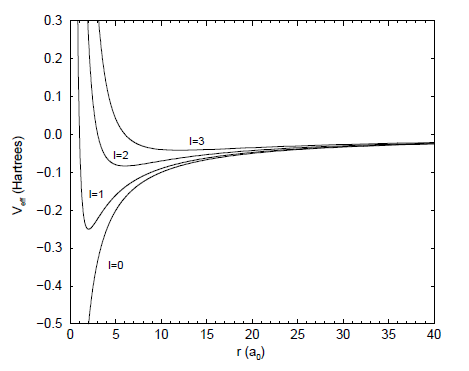
\includegraphics[scale=0.80]{Images2/rad.PNG}
    \caption{Potentiel effectif $V_\text{eff}$ pour Z=1}
    \label{fig:potentieleffectif}
\end{figure}
À courte distance, on observe que le terme en $\dfrac{1}{r^2}$ domine. Sans moment angulaire, on a juste un potentiel coulombien. En ajoutant un terme en $\dfrac{1}{r^2}$ (<<potentiel centrifuge>>, n'existe que quand on a un moment angulaire non nul) on obtient une barrière de potentiel à courte distance. Ainsi, le moment angulaire va empêcher l'électron d'approcher du noyau (c'est-à-dire du proton dans notre cas de l'hydrogène). On s'attend donc, lorsque qu'on va calculer la fonction d'onde radiale, à ce qu'elle soit localisée près du noyau lorsque $l=0$ et de plus en plus loin du noyau au fur et à mesure que $l$ grandit.


Il est possible de faire en sorte que l'équation soit plus simple et en unités réduites. Pour que le comportement colle avec ce qu'on sait déjà, il faut qu'à l'infini la probabilité de présence de l'électron tende exponentiellement vers 0, quelle que soit la valeur de $l$ car quand on s'éloigne, on atteint une zone où l'énergie totale est inférieure à l'énergie potentielle donc la probabilité de présence de l'onde dans cette zone doit tendre vers 0. C'est une région qui est classiquement interdite, mais tenant compte des effets tunnel, la fonction d'onde y est présente, mais décroît de façon exponentielle.


Posons, pour simplifier les notations, les quantités sans dimension

\[
    \rho\eq\left(-\dfrac{8\mu E}{\hbar^2}\right)^{1/2}r
\]

\begin{equation}
    \lambda\eq\dfrac{Ze^2}{4\pi\epsilon_0 \hbar}\left(-\dfrac{\mu}{2E}\right)^{1/2}\eq Z\alpha\left(-\dfrac{\mu c^2}{2E}\right)^{1/2}
    \label{lambda}
\end{equation}
où $\alpha=e^2/(4\pi\epsilon_0 \hbar c) \approx 1/137$ est la constante de structure fine. Cela nous permet de réécrire l'équation \eqref{jsp} comme


\begin{equation}
    \left[\ffdif{}{\rho}-\dfrac{l(l+1)}{\rho^2}+\dfrac{\lambda}{\rho}-\dfrac{1}{4}\right]u_{El}(\rho)\eq0
    \label{reduite}
\end{equation}
Lorsque $\rho \rightarrow +\infty$, les termes en $\dfrac{1}{\rho}$ et $\dfrac{1}{\rho^2}$ sont négligeables et alors les 2 solutions de \eqref{reduite} sont de la forme exp$(\pm \rho/2)$. Comme on cherche des solutions bornées, on ne garde que la solution asymptotiquement décroissante et donc on a la condition suivante sur notre solution:

\[
    u_{El}(\rho)\sim e^{-\rho/2} \quad \text{pour} \quad \rho \longrightarrow \infty
\]
Ainsi, la fonction $u_{El}(\rho)$ doit être de la forme

\[
    u_{El}(\rho)\eq e^{-\rho/2}f_{El}(\rho)
\]
avec $f_{El}(\rho)$ satisfaisant l'équation

\begin{equation}
    \left[\fdif{}{\rho^2}-\fdif{}{\rho}-\dfrac{l(l+1)}{\rho^2}+\dfrac{\lambda}{\rho}\right]f_{El}(\rho)\eq0
    \label{fel}
\end{equation}
De plus, quand $\rho \longrightarrow 0$, c'est le terme en $1/\rho^2$ qui devient dominant dans \eqref{reduite}. La solution régulière est de la forme

\[
    u_{El}(\rho) \sim \rho^{l+1} \qquad \text{pour} \qquad \rho \longrightarrow 0
\]
Supposons que $f_{El}(\rho)$ puisse s'écrire sous la forme

\[
    f_{El}(\rho)\eq\rho^{l+1}g_{El}(\rho)
\]
où on développe $g_{El}$ en série:

\[
    g_{El}(\rho)\eq\sum_{k=0}^{\infty} c_k\rho^k \quad c_0 \neq 0
\]
En injectant ce développement de solution dans \eqref{fel}, on obtient l'équation que doit satisfaire $g_{El}(\rho)$:

\begin{equation}
    \left[\rho\ffdif{}{\rho}+(2l+2-\rho)\fdif{}{\rho}+(\lambda-l-1)\right]g_{El}(\rho)\eq0
    \label{gel}
\end{equation}
En y substituant notre développement en série, on obtient la relation de récurrence que doivent satisfaire les coefficients $c_k$:

\begin{equation}
    c_{k+1}\eq\dfrac{k+l+1-\lambda}{(k+1)(k+2l+2)}c_k
\end{equation}
Supposons que $g_{El}(\rho)$ soit un polynôme de degré $n_r$. Comme il doit être fini, il faut que $c_{n_{r}+1}$=0 du coup

\[
    n_r+l+1-\lambda\eq0 \quad \Rightarrow \quad \lambda\eq n_r +l+1
\]
$\lambda$ est donc un nombre entier positif. On l'appelle nombre quantique principal de la solution et on le note $n$. La relation \eqref{lambda} fournit la valeur propre $E_n$ de la solution:

\begin{equation}
    E_n\eq -\dfrac{1}{2n^2}\left(\dfrac{Ze^2}{4\pi\epsilon_0}\right)^2\dfrac{\mu}{\hbar^2}\eq -\dfrac{1}{2}\mu c^2 \dfrac{(Z\alpha)^2}{n^2}
\end{equation}

Le spectre d'énergie de l'atome d'hydrogène (c'est-à-dire les valeurs de l'énergie pour différents $n$) est représenté à la figure \ref{fig:spectreH}.
\begin{figure}[htp]
    \centering
    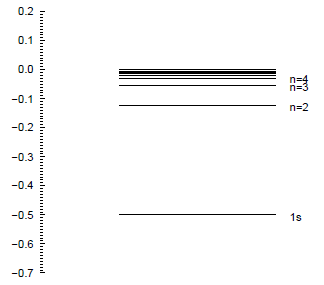
\includegraphics{Images2/spectreH.PNG}
    \caption{Spectre d'énergies de l'atome d'hydrogène. Les énergies sont exprimées en Hartree}
    \label{fig:spectreH}
\end{figure}
Pour chaque nombre quantique principal, on a un certain nombre de sous-niveaux qui est croissant avec $n$ (pour $n=1$ on a le niveau 1s, pour $n=2$ on a 2s et 2p...). Il y a donc une dégénérescence des niveaux d'énergie qui peuvent donc correspondre à des fonctions d'onde différentes, ce qui va compliquer le spectre. Cette dégénérescence est due (c'est non trivial) à la dépendance en $r^{-1}$ du potentiel coulombien et peut être levée par l'action d'un champ électrique ou magnétique (effets Stark et Zeeman).

Comme la puissance du polynôme $g_{El}$ vaut $n_r=n-l-1$ qui est forcément nul ou positif, il y a $n-1$ valeurs possibles de $l$ pour chaque valeur de $n$: $l=0, 1, ..., n-1$. De plus il y a $2l+1$ valeurs possibles de $m$ pour chaque valeur de $l$: $m=-l, -l+1, ..., l-1, l$. Le degré de dégénérescence du niveau $E_n$ vaut donc

\[
    \sum_{l=0}^{n-1} (2l+1)\eq 2\sum_{l=0}^{n-1} l + n \eq  2 \dfrac{(n-1)n}{2} + n \eq  n^2
\]
On remarque un tassement des niveaux vers la limite d'ionisation (région entre $n=2$ et $n=\infty$).

\subsection{Solution complète}
Il se trouve que les polynômes $g_{El}(\rho)$ sont des polynômes de Laguerre associés. En effet ceux-ci sont définis comme solutions de l'équation différentielle

\begin{equation}
    \left[x\ffdif{}{x}+(K+1-x)\fdif{}{x}+N\right] L_{N}^{K}(x)\eq 0
\end{equation}
L'équation \eqref{gel} est similaire à cette équation, et en les comparant on en déduit même que

\[
    g_{El}(\rho)\eq L_{n-l-1}^{2l+1}(\rho)
\]
En regroupant les résultats des sous-sections précédentes, on a donc comme solution pour les fonctions d'onde normalisées des états liés de l'atome d'hydrogène:

\begin{equation}
    \Psi_{nlm}(r,\theta,\phi)\eq -\left[\left(\dfrac{2Z}{na_{\mu}}\right)^3\dfrac{(n-l-1)!}{2n[(n+l)!]^3}\right]^{1/2}e^{-\rho/2}\rho^l L_{n-l-1}^{2l+1}(\rho)Y_{lm}(\theta,\phi)
    \label{sol}
\end{equation}
où on a remplacé l'indice $E$ par $n$ vu que ces 2 quantités sont reliées par une relation univoque.


\subsection{Étude des fonctions d'ondes radiales}
On souhaite développer quelques fonctions radiales pour les états les plus bas du spectre. On considère donc la partie radiale de \eqref{sol} dans laquelle on effectue l'approximation du noyau infiniment lourd ($\mu=m$). Ainsi $a_\mu$ se réduit à

\[
    a_{\mu}\eq \dfrac{4\pi\epsilon_0\hbar^2}{\mu e^2}\eq \dfrac{4\pi\epsilon_0\hbar^2}{me^2}\eq  a_0
\]
qui est le rayon de Bohr. De plus,

\[
    \rho\eq \dfrac{2Z}{n a_{\mu}}r
\]
En s'aidant d'une table contenant les polynômes de Laguerre \textbf{généralisés} (attention il y a les simples et les généralisés !), on obtient les fonctions radiales de la figure \ref{fig:foncrad} pour (dans l'ordre) les états 1s, 2s, 3s, 2p, 3p, 3d.

\begin{figure}[htp]
    \centering
    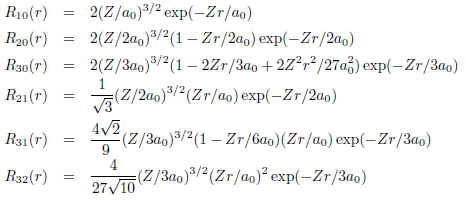
\includegraphics{Images2/foncrad.PNG}
    \caption{Fonctions radiales}
    \label{fig:foncrad}
\end{figure}
On remarque que les fonctions d'onde s ont une amplitude non nulle en $r = 0$, contrairement aux fonctions
d'onde des états $l\neq 0$ qui se comportent en $r^l$ près de l'origine. C'est le potentiel centrifuge $l(l+1)\hbar^2/2\mu r^2$ qui empêche l'électron de pénétrer dans le noyau. Pour une même valeur de n, les états de plus bas $l$ ont une amplitude plus importante près de $r = 0$.

À la figure \ref{fig:fcx_rad_1} sont représentées les fonctions d'onde radiales ($R_{nl}$) et fonctions de distribution radiales ($D_{nl}(r)=r^2|R_{nl}(r)|^2$) (qui est la probabilité par unité de longueur de trouver l'électron à une distance $r$ du noyau) de quelques états de l'atome d'hydrogène ($Z=1$):
\begin{figure}[htp]
    \centering
    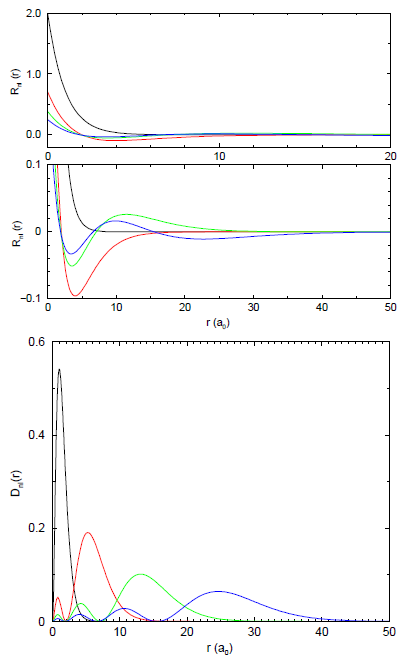
\includegraphics[scale=0.8]{Images2/ex.PNG}
    \caption{Fonctions d'onde radiale et de distribution radiale des 4 premiers états s. Le nombre de noeuds est $n-1$}
    \label{fig:fcx_rad_1}
\end{figure}
Quelques remarques à propos de ces figures:

\begin{itemize}[label=$\bullet$]
    \item Si on veut savoir quelle est la probabilité que l'électron se trouve à une distance $r$ du noyau, il faut prendre le carré de la fonction d'onde et intégrer sur le volume, cette probabilité de trouver l'électron dans une coque sphérique comprise entre $r$ et $r+\dif r$ est donc $r^2|R_{nl}(r)|^2\dif r\int \dif\Omega |Y_{lm}(\theta,\phi))|^2$. Il y aura donc apparition d'un facteur $r^2$ venant des coordonnées sphériques. Ce qu'on va calculer c'est donc la densité radiale de probabilité. L'intégrale porte aussi bien sûr sur la partie angulaire de la fonction d'onde, mais ce n'est pas ce qui nous intéresse. La densité radiale est en fait la probabilité de présence à une certaine distance $r$ du noyau.
    \item Dans un état 1s, l'électron se trouve à une distance moyenne d'un rayon de Bohr, par définition. Sa distribution est centrée à une unité atomique.
    \item Dans l'état 2s, la majeure partie de la probabilité se trouve à plus grande distance que pour l'état 1s. De 1 u.a. (pour 1s), on est passé à environ 4 u.a. (pour 2s).
    \item Le nuage électronique s'étend rapidement au fur et à mesure que $n$ augmente (évolution en $n^2$)
    \item La courbe de distribution radiale de l'état 1s montre un confinement tout près de $r=0$.
    \item On remarque la présence de lobes sur les courbes, le nombre changeant avec le moment angulaire: en effet les fonctions radiales dépendent de $l$.
    \item Les polynômes de Laguerre ont un indice $n-l-1$ et cet indice indique le nombre de noeuds de la fonction.
\end{itemize}

Les figures \ref{fig:fcx_rad_2} et \ref{fig:fcx_rad_3} sont quelques représentations des fonctions d'onde et distributions radiales pour d'autres états.

\begin{figure}[htp]
    \centering
    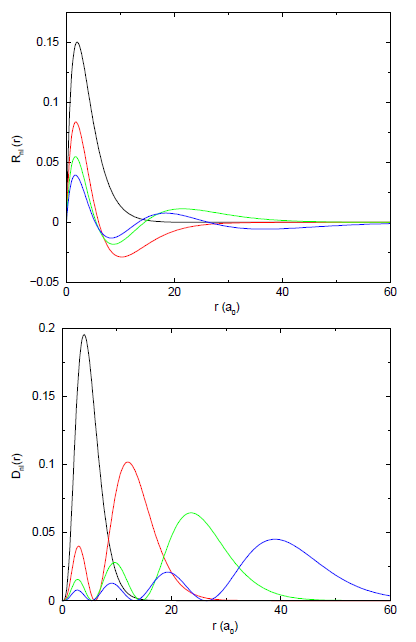
\includegraphics{Images2/p.PNG}
    \caption{Fonction d'onde radiale et fonction de distribution radiale des 4 premiers états p (courbe 2p bien centrée à 4 rayons de Bohr). La courbe noire correspond à 2p et la courbe bleue à 5p.}
    \label{fig:fcx_rad_2}
\end{figure}

\begin{figure}[htp]
    \centering
    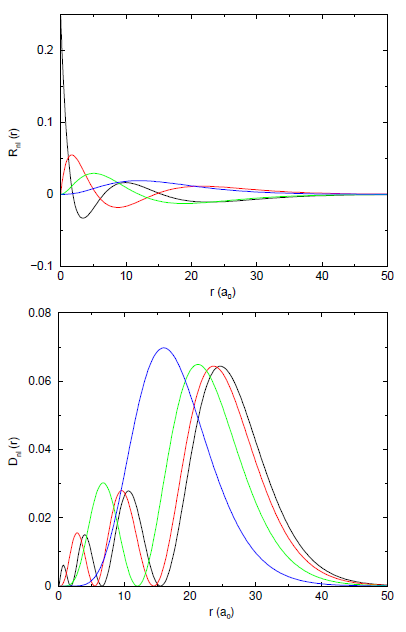
\includegraphics{Images2/spdf.PNG}
    \caption{Fonction d'onde radiale et fonction de distribution radiale des états 4s, 4p, 4d et 4f. Le nombre de noeuds est $4-l-1$}
    \label{fig:fcx_rad_3}
\end{figure}

Les états de moment angulaire maximum ($l=n-1$) sont beaucoup plus simples à comprendre que les autres qui ont un comportement ondulatoire (présence de noeuds et ventres dans leur fonction d'onde). En effet, l'électron peut être vu comme une onde piégée dans un potentiel qui va, sous l'action de ce dernier, former une espèce d'onde stationnaire : ce sont les noeuds et les ventres que l'on observe (l'électron a une probabilité de présence nulle sur un noeud et une probabilité forte sur un ventre). On peut donner une image assez classique de ces noeuds et ventres. Lorsqu'on a des noeuds et des ventres, on peut voir l'électron comme une onde stationnaire qui fait des allers-retours entre le noyau et le bord du potentiel. Cependant, lorsque $l$ est maximal (i.e. $l=n-1$), la partie radiale de la fonction d'onde $R_{n,l=n-1}$ ne présente plus qu'un seul ventre sans noeuds. Dès lors, on doit ainsi plus voir l'électron comme orbitant à une distance moyenne constante du noyau. Attention que ceci est une image fort classique pour la mécanique quantique. Cependant plus $n$ est grand, plus on se rapproche de cette image et on peut donc considérer l'électron comme étant une particule classique orbitant autour d'un noyau (surtout à partir de $n=100$).

Plus le nombre quantique $n$ d'un état est élevé, plus l'état correspondant est excité. Un état de grand $n$ est appelé état de Rydberg. À l'échelle atomique, la fonction d'onde d'un tel état s'étend sur de très grandes distances, comme suggère l'expression du maximum de la fonction de distribution radiale

\[
    r\eq \dfrac{n^2}{Z}a_{\mu}
\]
Par exemple, la fonction d'onde radiale de l'état 50s qui est représentée figure \ref{fig:50s} s'étend jusque $5000a_0= \SI{0.27}{\mu m}$.

\begin{figure}[htp]
    \centering
    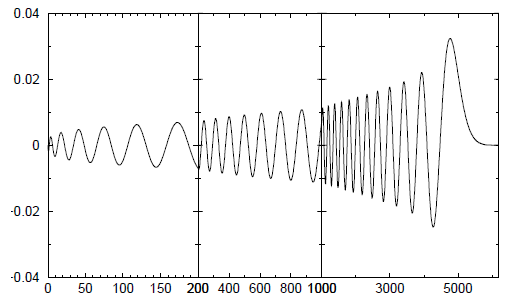
\includegraphics{Images2/50s.PNG}
    \caption{Fonction d'onde radiale réduite de l'état 50s}
    \label{fig:50s}
\end{figure}



\newpage
\section{Systèmes à électrons non appariés}
\subsection{Introduction : les alcalins}
Les alcalins sont les éléments de la première colonne du tableau périodique. Ils ont une structure électronique à coeur de gaz rare. Ils perdent facilement leur électron de valence célibataire dans la sous-couche externe s. Nous avons par exemple:

\begin{center}
    Li [He:1s$^{2}$] 2s \\
    Na [Ne: 1s$^{2}$2s$^{2}$2p$^{6}$] 3s \\
    K [Ar: 1s$^{2}$2s$^{2}$2p$^{6}$3s$^{2}$3p$^{6}$] 4s
\end{center}
Pour chaque sous-couche pleine, on rappelle qu'on a $\sum_i l_i = 0$.

Nous allons essayer de décrire ces atomes comme un atome d'hydrogène. Tout d'abord, nous nous intéressons au lithium. Dans cette approche de l'atome d'hydrogène, on peut voir l'électron 2s comme lié à un ion Li$^{+}$ que l'on peut considérer approximativement comme un proton dans le sens où c'est une charge positive. Puisque c'est un électron 2s, nous savons qu'il a une probabilité de présence non nulle près du noyau, c'est-à-dire dans le volume occupé par les deux autres électrons.


Étant donné que tout cela est probabiliste, il se peut que l'électron 2s se trouve plus proche du noyau que les autres électrons (<<plus proche>> d'une façon tout à fait schématique) et que donc il <<voit>> une charge qui n'est pas, $1e$ mais $2e$ ou, $3e$ car il n'y a plus d'effet d'écrantage.

Nous avons donc $Z$ qui augmente et l'énergie de liaison $E_n \propto 1/n^2$ aussi. Nous corrigeons par conséquent le nombre quantique principal qui n'est donc plus un nombre entier. Cette correction s’appelle le \textbf{défaut quantique}, notée $\delta_l$, et c’est une bonne solution pour décrire la perturbation de ces électrons dits externes lorsque nous faisons varier le nombre quantique principal.
Le défaut quantique sera toujours du même ordre de grandeur pour tous les alcalins, car il ne dépend pas de, $n$ mais seulement de $l$. En effet, la probabilité de présence près du noyau de l'électron diminue avec l'augmentation de $l$, donc le défaut quantique sera plus grand pour les plus petits $l$. Pour des moments angulaires plus importants ($l$ élevé), le potentiel effectif (dû au terme centrifuge) va empêcher les électrons externes d’aller à courtes distances et donc ils ne seront pas perturbés par la présence des autres électrons.

\[
    \delta_s>\delta_p>\delta_d>\delta_f\simeq 0
\]
L'énergie de liaison des alcalins obéit à la loi de Balmer modifiée par l’introduction du défaut quantique, qui rend compte de l’écrantage imparfait de la charge du noyau par les autres électrons. Il est d’autant plus grand que l’orbitale a une grande probabilité de présence à courte distance.

\begin{equation}
    E_{nl} \eq  - \dfrac{Ry}{2(n-\delta_l)^2}
    \label{eq:def_quant}
\end{equation}

NB: pas de facteur 2 au dénominateur quand on est en eV ; on est en Hartree dans cette formule.


Si nous nous intéressons maintenant au cas du sodium nous constatons que la correction dépasse 1 pour $l=0$ : $\delta_l = 1.35$. Cela signifie que le remplissage des couches ne se fera pas suivant la règle de Madelung (ou  Klechkowski). \textcolor{red}{Sûr de ça? Parce qu'il y a aussi l'effet joué par la correction du terme $l=1$ à prendre en compte si on veut `classer' les couches}
En effet, pour le potassium (K) par exemple, le 3 de la sous-couche 3d devient 2.75 tandis que le 4 de la sous-couche 4s devient 1.81. Par conséquent, l’énergie de la 4s est plus petite que celle du 3d comme l'indique la formule \ref{eq:def_quant}. La sous-couche 4s sera donc remplie avant la 3d.

Ce phénomène ne se limite pas seulement aux alcalins. Pour  n'importe quel atome excité, nous pouvons calculer le défaut quantique. (cf. exercice sur l'hélium vu en TP).




\subsection{Rayon X}
\subsubsection{Contexte et rappels}


Nous allons ici développer un outil très important pour l'identification des éléments. Il a notamment servi à identifier la présence d'éléments terrestres dans le Soleil, ce qui n'avait a priori rien d'évident. En bombardant un matériau d'électrons de haute énergie, on observe l'émission de rayons X caractéristiques de sa structure.\\

Dans un atome à plusieurs électrons, nous savons que l'énergie ne suit plus exactement la loi de Balmer obtenue pour l'atome d'H ($E_n \propto Z/n^2$). En effet, il y a un effet dû aux autres électrons. Comme nous l'avons vu, cet effet peut être pris en compte en considérant un `défaut quantique' (formule \ref{eq:def_quant}). Cependant, une autre façon de voir les choses est d'utiliser une charge effective, mais de laisse le nombre quantique inchangé. Cette charge effective $Z^{*}$ perçue par chaque électron est définie comme \[ Z^{*}=Z-\sigma \] où $\sigma$ représente l'effet d'écran produit sur l'électron d'intérêt par les électrons plus proches du noyau. Dès lors, l'énergie s'exprime comme

\begin{equation}
    E_n \eq -\dfrac{1}{2} \dfrac{(Z-\sigma_n)^2}{n^2} \; [\si{ua} = \si{Ha}]
    \label{eq:energie_effective}
\end{equation}
Comme vu dans l'introduction, lors du passage d'un électron de haute énergie dans un milieu matériel, l'électron subit une perte d'énergie continue sous forme de rayonnement de freinage (pour de hautes énergies de l'électron incident, on peut ignorer la perte sous forme d'ionisation, voir figure \ref{fig:Résumé pertes}). La figure idéalisée de ce rayonnement selon la longueur d'onde de l'électron incident\footnote{On observe donc bien entendu pour un même électron une variation de cette longueur d'onde au cours de sa progression.} se trouve à la figure \ref{fig:Freinage idéalisé} où l'\textit{intensité relative} correspond à l'intensité du rayonnement, autrement dit $\fdif{E}{x}$ la perte d'énergie par unité de distance pour l'électron [\si{J/m}].

\begin{figure}[htp]
    \centering
    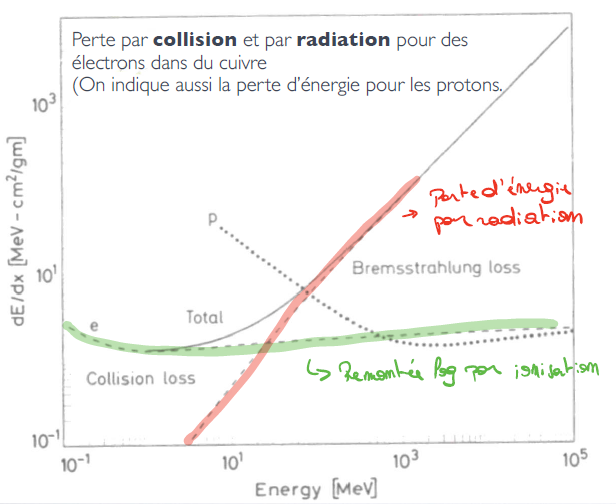
\includegraphics[scale=0.8]{Images2/RésuméPerte.PNG}
    \caption{Perte d'énergie par unité de longueur en fonction de l'énergie incidente. On a ici représenté les 2 effets de perte d'énergie dans un matériau : le rayonnement de freinage et la perte par ionisation}
    \label{fig:Résumé pertes}
\end{figure}%
\begin{figure}[htp]
    \centering
    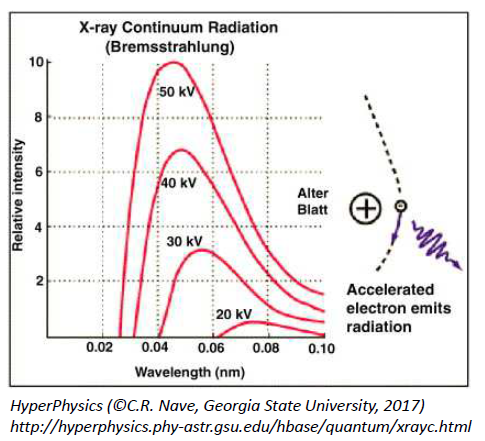
\includegraphics[scale=1.0]{Images2/FreinageIdéalisé.PNG}
    \caption{Rayonnement de freinage sans phénomène de résonance avec les atomes de la cible}
    \label{fig:Freinage idéalisé}
\end{figure}%

Dans la réalité, la perte d'énergie par unité de longueur en fonction de la longueur d'onde incidente est du type de la courbe représentée à la figure \ref{fig:Rayonnement freinage} (et non de la courbe représentée à la figure \ref{fig:Freinage idéalisé} qui n'est qu'une approximation négligeant complètement un phénomène important). Ainsi, pour des longueurs d'onde particulières, la perte d'énergie est drastiquement augmentée. Le phénomène responsable de cette perte drastique est dû à la résonance entre l'énergie de l'électron incident et (dans notre cas présent) des électrons de coeur : l'énergie perdue par les électrons lors de cette résonance correspond à l'énergie des photons associés aux rayons X observés dont nous discuterons dans un instant.\\
\begin{figure}[htp]
    \centering
    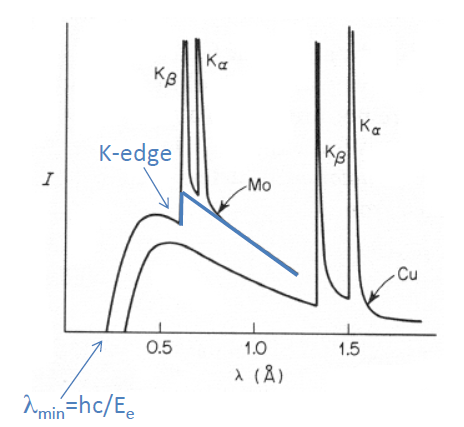
\includegraphics[scale=1.0]{Images2/RayonnementFreinage.PNG}
    \caption{Rayonnement de freinage avec résonance avec les niveaux profonds des atomes cibles}
    \label{fig:Rayonnement freinage}
\end{figure}


\subsubsection{Émission de rayons X}


Les fréquences auxquelles on observe les phénomènes de résonance dans le spectre du rayonnement de freinage (= les fréquences où on a des pics d'absorption) correspondent aux fréquences des transitions d'orbitales $n = 2$ vers $n = 1$. Pour caractériser ces transitions, on peut se servir de la loi empirique de Moseley, qui n'est qu'une généralisation des différentes séries de Lyman, Balmer, etc\footnote{En fait, on peut l'obtenir en faisant simplement la différence entre deux niveaux d'énergie distincts via la formule \ref{eq:energie_effective} où on considère un écrantage `moyen' (=la moyenne des écrantages des deux niveaux dont on fait la différence).}.
\begin{equation}
    h\nu
    \eq E_{n_1} - E'_{n_2}
    \eq \dfrac{1}{2}(Z-\sigma_{n_1})^2\left(\dfrac{1}{n_1^2}-\dfrac{1}{n_2^2}\right)
    \label{eq:Moseley}
\end{equation}

Mais dis-moi Jamy, pourquoi est-ce que les atomes émettent ces rayons X? Hé bien Fred, c'est très simple : lors du passage de la particule incidente dans l'atome, on va observer des chocs entre elle et les électrons de coeur (de $n=1$ voire $n=2$) qui sont fortement liés au noyau (en effet, les électrons proches du noyau ne subissent aucun effet d'écrantage atténuant l'action du noyau). Ces chocs avec les électrons de coeur entraînent des trous dans la couche qui sera comblée par la transition d'un électron d'une couche de $n$ plus élevé ($n=2$ sur la figure \ref{fig:Rayons X}). Le rayon X est donc l'émission qui s'associe au passage de l'électron d'une orbitale d'un $n$ élevé à l'orbitale de coeur qui a perdu un électron.
\begin{figure}[htp]
    \centering
    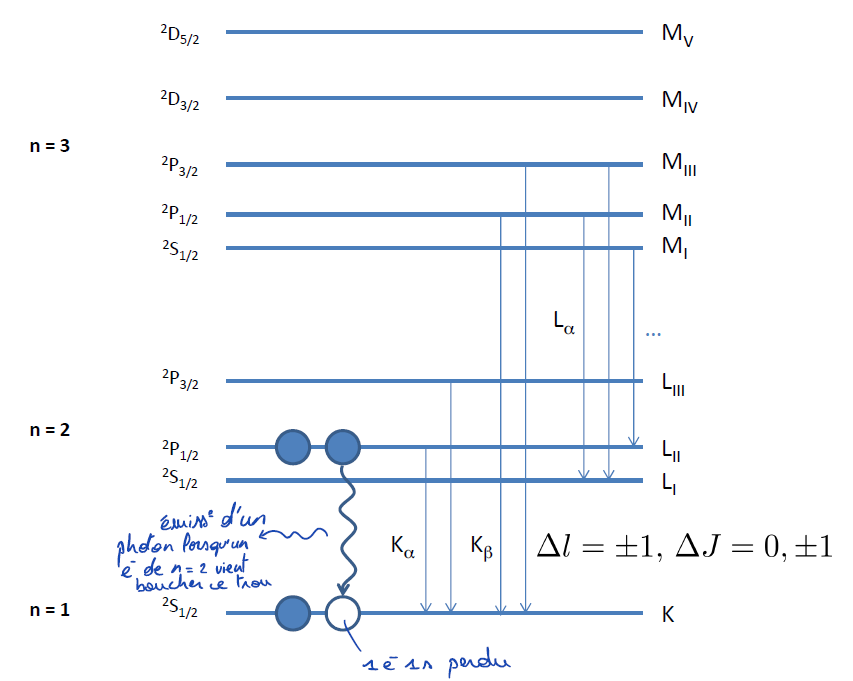
\includegraphics[scale=0.8]{Images2/Rayons X.PNG}
    \caption{Schéma de l'émission de rayons X suite à une ionisation de coeur.}
    \label{fig:Rayons X}
\end{figure}
Grâce aux rayons X, on peut calculer l'effet d'écran d'une certaine couche, c'est-à-dire <<de combien la charge du noyau diminue-t-elle quand on se trouve au-delà de cette couche et donc que les électrons de cette couche agissent comme un écran?>>. Lors d'une ionisation depuis $n=1$, on a deux électrons dans la couche s1 et donc l'écrantage est approximativement 2. Après ionisation, il ne reste plus qu'un seul électron dans cette couche et par conséquent l'effet d'écran n'est plus que 1 approximativement : Z est à peu près diminué de 1. Ainsi, l'ionisation a bien diminué l'effet d'écran de 1.\\
Pour ce qui est des ionisations de la couche (complète : 8 électrons) $n=2$, on observe après ionisation un effet d'écran de 7.4 dans cette couche de 7 électrons, ce qui est cohérent. Ces valeurs de correction ont été découvertes empiriquement (cf. l'équation de Moseley \ref{eq:Moseley}).
On calcule donc les fréquences des photons associées aux transitions $2\rightarrow1$ et $3\rightarrow2$:
\[
    \nu_{12}
    \eq \nu_{K_\alpha}
    \eq k (Z - 1)^2 \;[Hz]
\]
\[
    \nu_{23}
    \eq \nu_{L_\alpha}
    \eq k' (Z - 7.4)^2 \;[Hz]
    \;\approx\;  k' (Z - 7)^2 \;[Hz]
\]
où $k$ et $k'$ sont des constantes numériques issues de la formule \ref{eq:Moseley}.



\subsubsection{Émission d'électrons \emph{Auger}}



On sait par la formule \ref{eq:Moseley} que la différence d'énergie entre le seuil d'ionisation et le niveau $n = 2$ est toujours inférieure à la différence d'énergie entre les niveaux 1 et 2. Intéressons-nous à l'émission des <<électrons Auger>>, comme représenté à la figure \ref{fig : Auger}. En fait, lorsqu'un rayonnement ionisant ionise l'électron $1s$, les électrons des couches externes vont venir boucher ce trou en émettant des rayons X. Or, comme rappelé au début de ce paragraphe, l'énergie entre 1s n'importe quel autre niveau est supérieure à l'énergie d'ionisation d'un électron d'un niveau de $n>2$.

Dès lors, dans notre exemple à la figure \ref{fig : Auger}, le rayon X libéré par l'électron $^2P_{1/2}$ a une énergie suffisante pour ioniser l'autre électron $^2P_{1/2}$. Cet autre électron, ionisé, est appelé <<électron Auger>> et peut en pratique se situer n'importe où ailleurs dans l'atome (il ne se trouve pas forcément au même terme que l'électron qui bouche la couche 1s). Ainsi, on se retrouve avec un atome ayant perdu 2 électrons au total. En outre, on peut avoir 3 électrons manquant à la fin si le rayonnement provoqué par l'ionisation de l'électron Auger ionise encore un autre électron (ce phénomène est moins intense cependant).

Il est dès lors probable que, à la place d'émettre un rayon X, notre atome émette un électron. Cet électron émis aura l'énergie du rayon X (qui est la différence entre les niveaux d'énergie) diminuée du potentiel d'ionisation. On peut ainsi observer un spectre de fréquence à la figure \ref{fig:SpectreAuger} pour ces électrons émis, et ce spectre est structuré de la même façon que le spectre d'émission des rayons X. En fait, la seule différence entre le spectre d'émission d'électrons et le spectre d'émission de rayons X par un atome soumis à un rayonnement ionisant est le potentiel d'ionisation : les électrons doivent effectuer un travail pour sortir de la matière, contrairement aux photons.
\begin{figure}[htp]
    \centering
    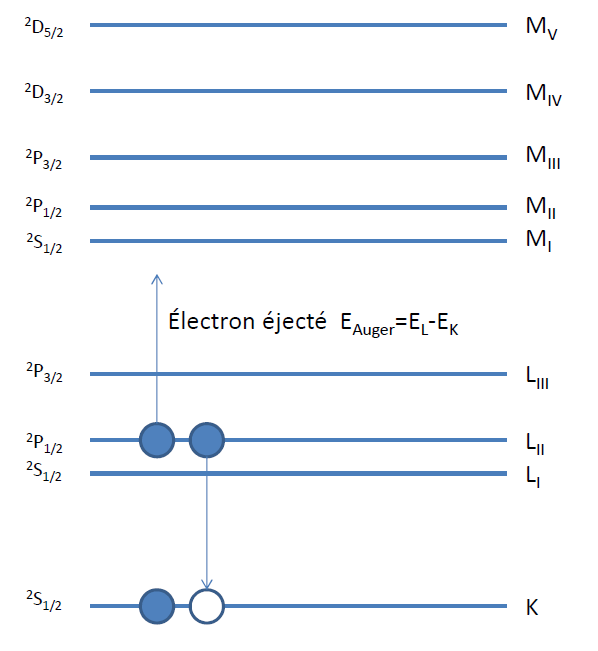
\includegraphics[scale=0.8]{Images2/Auger.PNG}
    \caption{Schéma de l'émission d'électrons Auger suite à une ionisation de coeur.}
    \label{fig : Auger}
\end{figure}
\begin{figure}[htp]
    \centering
    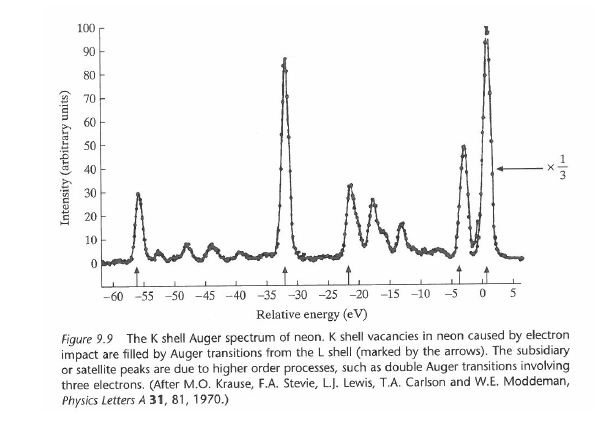
\includegraphics[scale=1.0]{Images2/Spectre Auger.PNG}
    \caption{Spectre en fréquence des électrons Auger}
    \label{fig:SpectreAuger}
\end{figure}








\subsection{Le laser}

\subsubsection{Émission spontanée, émission et absorption stimulées}




On détaille ici les équations qui gouvernent ces phénomènes. L'analogie avec la cinétique chimique pour des réactions d'ordre 1 ou la radioactivité est directe. <<Un atome ne vieillit pas>> et un état non plus, la probabilité de transition par unité de temps est donc une constante.\\
Nous allons donc dans cette section décrire les différents phénomènes d'émission et d'absorption à l'aide d'équations différentielles. Nous allons également utiliser des taux de transitions $A_{ij}$ et $B_{ij}$ (= probabilité de transition par seconde) tels que $i$ est l'état de départ et $j$ l'état d'arrivée.
\begin{figure}[htp]
    \centering
    \includegraphics[scale=0.8]{Images2/Emission Spontanée.PNG}
    \label{fig:emission_spont}
\end{figure}
où $N_2(t)$ est la population atomique dans l'état d'énergie $E_2$.
\begin{figure}[htp]
    \includegraphics[scale=0.85]{Images2/Absorption stimulée.PNG}
    \label{fig:absorb_stimul}
\end{figure}
\begin{figure}[htp]
    \includegraphics[scale=0.9]{Images2/Emission stimulée.PNG}
    \label{fig:emission_stimul}
\end{figure}
Avant de continuer, quelques remarques :
\begin{itemize}[label=$\bullet$]
    \item L'émission `spontanée' n'existe pas vraiment. En effet, il faut toujours qu'il y ait une excitation qui pousse un électron à émettre un rayonnement. Ce qu'on dénote par <<émission spontanée>> est l'émission d'un photon par l'électron sous une excitation interne à l'atome (pas de photon externe à l'atome venant l'exciter). Ces photons <<internes>> sont les photons du champ E : selon la QED, le champ EM est composé de photons virtuels et ce sont ces photons virtuels qui excitent nos électrons.
    \item L'émission stimulée, bien que contre-intuitive, découle simplement de la micro réversibilité de l'absorption stimulée : Einstein savait que la physique aimait la <<micro-réversibilité>> et il devait par conséquent avoir un phénomène opposé à l'absorption stimulée.
    \item Pour ce qui est des émissions (stimulée comme spontanée), on se rend bien compte que la solution à l'équation différentielle sera une exponentielle décroissante avec le temps. D'une certaine population, on va avoir une atténuation exponentielle avec un temps de vie caractéristique qui est l'inverse de la constante $A_{ij}$ ou $B_{ij}$. Ceci n'est valide que lorsqu'on a uniquement de l'émission stimulée ou uniquement de l'émission spontanée.
    \item On a ici décomposé l'élément de la matrice de perturbation associé aux états concernés $W_{ij}(\nu)$ en un facteur indépendant de l'onde incidente $B_{ij}$ et la densité d'énergie incidente $\rho(\nu)$.
    \item On n’a pas de relation à ce stade entre $B_{12}$ et $B_{21}$.
\end{itemize}
On peut exprimer, de manière tout à fait générale, l'évolution des populations\footnote{Le terme `population' désigne le nombre de particules dans un certain état dans un système. Plus précisément on parle dans notre cas d'une population d'électrons ayant la même énergie dans un gaz macroscopique par exemple.} en fonction des taux de transition ($A_{ij}$ et $B_{ij}$) et de la densité énergétique ($\rho(\nu)$).\\
En effet, dans un système à deux états, l'évolution de la population $N_1$ est dictée par son approvisionnement depuis l'état 2 (émissions spontanée et stimulée) en même temps que sa dépopulation pour aller vers l'état 2 (absorption stimulée):
\begin{equation}
\boxed{
    \fdif{N_1}{t}
    \eq  [B_{21}\rho(\nu) + A_{21}]N_2 \;-\; B_{12} \rho(\nu)N_1
    }
    \label{eq:N2}
\end{equation}
De façon tout à fait équivalente pour $N_2$, la population de l'état 2:
\begin{equation}
\boxed{
    \fdif{N_2}{t}
    \eq - [A_{21} + B_{21} \rho(\nu)]N_2 \;+\; B_{12}\rho(\nu)N_1
    \label{eq:N1}
    }
\end{equation}
En sommant les équations \ref{eq:N1} et \ref{eq:N2}, on observe bien la conservation du nombre de particules (du nombre d'électrons pour nous). Ceci se généralise très facilement lorsqu'on a plus que 2 états.
\begin{equation}
\boxed{
    \fdif{N_1}{t}\;+\;\fdif{N_2}{t} \eq 0
    }
\end{equation}



\subsubsection{L'équilibre thermodynamique}



Grâce à la théorie quantique du corps noir (on n'a plus l'évolution en $T^4$ de l'intensité en fonction de la longueur d'onde), on peut écrire l'expression de la densité énergétique \textbf{à l'équilibre thermodynamique} émise par une matière chauffée à une température $T$ donnée en fonction de la fréquence émise $\nu$. (Fig. \ref{fig:corps_noir})

\begin{equation}
    \rho(\nu) \eq \dfrac{8\pi h \nu^3}{c^3(\exp(\dfrac{h\nu}{k_BT})-1)}
\end{equation}
\begin{figure}[htp]
    \centering
    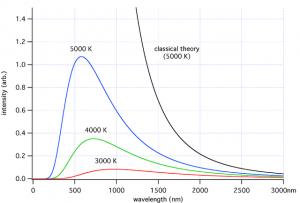
\includegraphics[scale=1.1]{Images2/corps_noir.png}
    \caption{Spectre d'un corps noir à diverses températures}
    \label{fig : Corps noir}
\end{figure}
Nous savons que la répartition entre les états 1 et 2 doit respecter la distribution de Maxwell-Boltzmann en prenant en compte les dégénérescences en énergie. Ces dégénérescences sont notées $g_1$ et $g_2$. L'excitation depuis l'état fondamental 1 vers l'état excité 2 qui est plus probable se fait thermiquement (via l'énergie $k_BT$) et est d'autant plus probable que $h\nu$, la différence d'énergie entre l'état 1 et l'état 2, est petite :
\[
    N_2 \eq \dfrac{g_2}{g_1} \; \exp\left(\dfrac{-h\nu}{k_BT}\right) \;N_1
\]
En partant des conditions d'équilibre thermodynamique et en substituant, on obtient :
\[
    \fdif{N_1}{t} \eq \fdif{N_2}{t} \eq 0
\]
\[
    \fdif{N_2}{t}
    \eq 0
    \eq - \left[\;A_{21} + B_{21} \rho(\nu) + B_{12}\rho(\nu) \dfrac{g_1}{g_2} \; \exp\left(\dfrac{h\nu}{k_BT}\right) \;\right] N_2
\]
\[
    \rho(\nu)
    \eq \dfrac{A_{21}}{B_{12}\rho(\nu) \cdot \dfrac{g_1}{g_2} \exp(\dfrac{h\nu}{k_BT}) - B_{21}}
    \;\equiv\; \dfrac{8\pi h \nu^3}{c^3\left(\exp(\dfrac{h\nu}{k_BT})-1\right)}
\]
Cette dernière égalité n'est pas triviale : en effet, nous égalisons la densité d'énergie classique obtenue avec la théorie du corps noir et la densité d'énergie du rayonnement. On peut aisément comprendre cette égalité en considérant le gaz compris dans un corps noir : à l'équilibre thermodynamique, l'énergie thermique transmise de la paroi à nos atomes est égale à l'énergie émise par rayonnement des atomes.\\
En isolant les taux de transition, on obtient ces deux relations qui seront très utiles.
\begin{equation}
    B_{21} \eq \dfrac{g_1}{g_2}B_{12}
    \label{eq:equilire1}
\end{equation}
\begin{equation}
    \dfrac{A_{21}}{B_{21}}
    \eq \dfrac{8\pi h \nu^3}{c^3}
    \eq \dfrac{\hbar \omega^3}{\pi^2c}
    \label{eq:equilire2}
\end{equation}
On remarque donc que pour un $A_{21}$ important par rapport à $B_{21}$, l'émission de lumière ultraviolette est bien plus probable que l'émission d'infrarouge.


\subsubsection{Principe de fonctionnement du LASER et inversion de population}



\begin{figure}[htp]
    \centering
    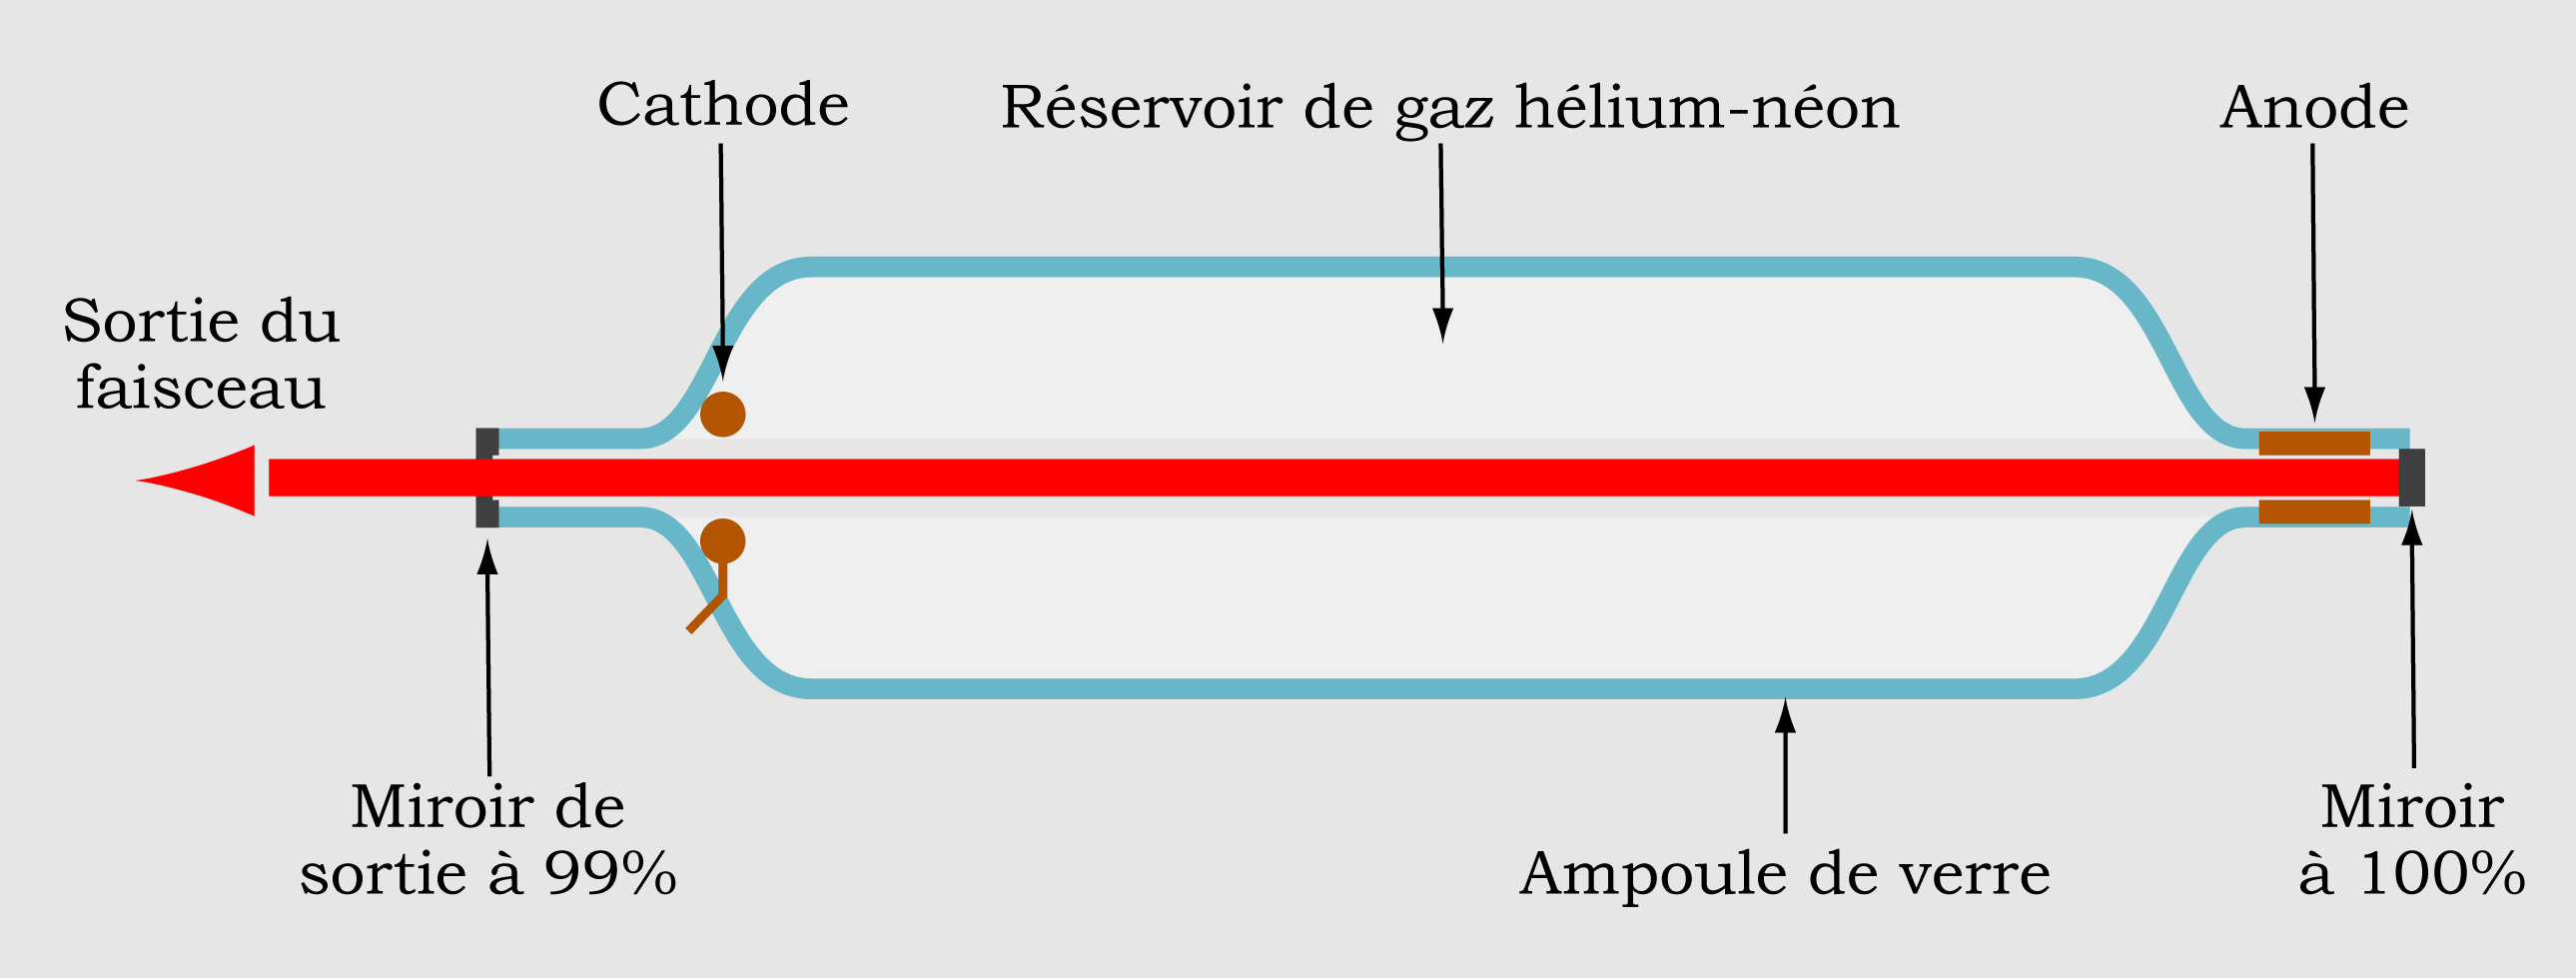
\includegraphics[scale=0.7]{Images2/Laser.png}
    \caption{Schéma d'un laser à hélium-néon}
    \label{fig:Laser}
\end{figure}
Le concept du laser est relativement simple : en se servant de l'émission stimulée, on met en place une réaction en chaîne qui transformera l'énergie fournie au système (via le courant créé par les électrodes) en émission de lumière dans une gamme extrêmement précise de fréquences. En pratique, l'amplification se fait dans la chambre à gaz, la lumière se propage selon l'axe $z$ jusqu'à un miroir à 99\% qui permet de laisser sortir une partie du faisceau (celle dont on se sert) et de réfléchir le reste dans le système pour à nouveau l'amplifier.

On s'était permis plus tôt une hypothèse simplificatrice que l'on ne peut conserver : on avait supposé que les états absorbaient de la lumière à toutes les fréquences. C'est le cas pour un solide cristallin possédant suffisamment d'états (de degrés de liberté), mais c'est faux pour un gaz dont les fréquences d'absorption sont celles des atomes : il n'y a pas de forme macroscopique dans un gaz pour créer beaucoup de niveaux d'énergie. Pour remédier à cela, nous introduisons une fonction $g(\nu - \nu_0)$ qui doit représenter l'atténuation de la stimulation dès qu'on s'éloigne de la fréquence de résonance $\nu_0$. On repart des équations \ref{eq:N1} et \ref{eq:N2} et des relations qu'on a trouvées grâce à l'équilibre thermodynamique \ref{eq:equilire1} et \ref{eq:equilire2}. On réécrit cependant les taux de transition $A_{ij}$ et $B_{ij}$ avec $\tau_{sp}$, le temps de vie de l'état 2:
\[
    \dfrac{g_1}{g_2}W_{12} \eq W_{21}^{st} \eq B_{21} \rho(\nu) g(\nu - \nu_0)
\]
\[
    W_{21}^{sp} \eq A_{21} \eq \dfrac{1}{\tau_{sp}} \eq \dfrac{8\pi \nu^3}{c^3}B_{21}
\]
\[
    W_{21}^{st} \eq \dfrac{c^3}{8\pi h \nu^3}\dfrac{\rho(\nu) g(\nu - \nu_0)}{\tau_{sp}}
\]
Intéressons-nous maintenant au rayon qui traverse notre gaz. On peut facilement imaginer que le phénomène d'amplification aura une forme exponentielle : une réaction émet $x$ photons qui donneront lieu à $x$ émissions stimulées.\\

On définit un facteur d'amplification $\gamma\ [\si{m^{-1}}]$, un gain qui représentera le comportement de notre faisceau le long de l'axe z (ou, de façon équivalente, au cours du temps via $c\dif t = \dif z$). On exprime également l'intensité lumineuse $I\ [\si{W/m^2}]$ comme un flux d'énergie à travers une surface, ce qui revient à multiplier la densité énergétique $\rho(\nu)\ [\si{J/m^3}]$ par la vitesse de propagation $c\ [\si{m/s}]$:
\[
    \fdif{I_\nu}{z} \eq \dfrac{\dif I_\nu}{c\dif t} \eq \gamma I_\nu
\]
\[
    I_\nu(z) \eq I_\nu(0) e^{\gamma z} \eq c\rho(\nu)
\]
%pas sûr d'avoir très bien compris comment intégrer la dépendance en z dans l'expression avec rho mais grosso modo c'est ça
On a ici négligé l'émission spontanée, elle a pourtant bien lieu, mais son caractère isotrope l'empêche de contribuer significativement au mécanisme. Il s'agit néanmoins d'une limitation technique qui entraîne une perte pour le système en fonctionnement.
Pour avoir un gain, il nous faut donc une augmentation du nombre de photons, on exprime donc la variation du nombre de photons par unité de volume [\si{1/m^3}], $N_{ph}$, au cours du temps. On a deux contributions à la variation de $N_{ph}$ : l'émission depuis l'état 2 vers l'état 1 (terme positif) et l'absorption depuis l'état 1 vers l'état 2 (terme négatif).
\[
    \fdif{N_{ph}}{t}
    \eq N_2 W_{21}^{st} - N_1 W_{12}
    \eq W_{21}^{st} (N_2 - \dfrac{g_2}{g_1}N_1)
\]
La variation de la densité énergétique au cours du temps est la variation du nombre de photons multipliée par l'énergie d'un photon. On passe ensuite à l'intensité via la vitesse de propagation $c$.
\begin{align*}
    \dfrac{1}{c}\fdif{I}{t}
    &\eq  \fdif{\rho}{t}\\
    &\eq  h\nu\fdif{N_{ph}}{t}\\
    &\eq  h\nu (N_2 - \dfrac{g_2}{g_1}N_1) \dfrac{c^3}{8\pi h \nu^3}\dfrac{\rho(\nu) g(\nu - \nu_0)}{\tau_{sp}}\\
    &\;\equiv\;  c\rho(\nu)\gamma
\end{align*}
En définitive, nous obtenons l'expression suivante pour le facteur d'amplification $\gamma$ :
\begin{equation}
    \boxed{
        \gamma \eq \dfrac{c^2}{8\pi\nu^2}\dfrac{g(\nu - \nu_0)}{\tau_{sp}}(N_2 - \dfrac{g_2}{g_1}N_1)
    }
\end{equation}
\[
\boxed{
    \gamma > 0 \; \longrightarrow \; \dfrac{N_1}{g_1} < \dfrac{N_2}{g_2}
    }
\]
On s'aperçoit donc que pour avoir une amplification du faisceau, il nous faut inverser les populations 1 et 2\footnote{Selon Wikipédia, \textit{une inversion de population se produit lorsqu'un système [...] se trouve dans un état dans lequel la majorité des éléments sont dans un état excité plutôt que dans leur état fondamental}}. Augmenter le courant ne ferait qu'échauffer le gaz qui suit la distribution de Maxwell-Boltzmann : cette dernière contraint la population de l'état fondamental à être au moins autant peuplée que tout autre état\footnote{Pour s'en convaincre, on peut se souvenir du modèle à deux états de la physique statistique pour lequel une température infinie entraîne une probabilité d'occupation de $\dfrac{1}{2}$ pour chaque état.}. On va donc devoir tricher.


\subsubsection{L'inversion de population en pratique}


La subtilité réside ici dans les petits termes en bas du contrat : cette limitation n'est valable en l'état que pour un système homogène\footnote{Sous-entendu : composé d'un seul type de corps}. On va donc choisir un mélange de gaz pour remplir notre laser, et comme souvent en science on ne va pas faire les choses au hasard.\\

Pour expliquer l'inversion de population, l'auteur, dans sa grande sagesse, a choisi une analogie claquée au sol. Imaginons avoir un escalier et un ensemble de billes. Imaginons que par la décision d'un Dieu mesquin ou d'une loi de la Nature quelconque, le nombre de billes par marche aille toujours décroissant alors qu'on monte dans les marches. Autrement dit, pour toute marche, la marche supérieure doit toujours contenir moins de billes (ou autant) que la marche du dessous.

\begin{figure}[htp]
    \centering
    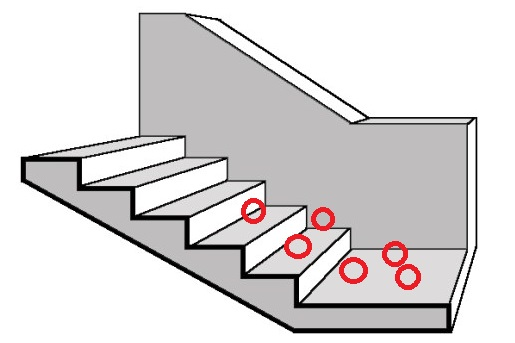
\includegraphics[scale=1.0]{Images2/escalier2.jpg}
    \caption{Un joli petit escalier}
    \label{fig:escalier}
\end{figure}
Imaginons maintenant que, bravant la volonté divine, on amène une échelle (= une grosse marche à côté de l'escalier) d'où l'on fait monter des billes. Dès lors, on se retrouve avec plus de billes sur la marche desservie par cette échelle que sur la marche d'en dessous : nous ne sommes plus à l'équilibre. Par conséquent, les billes vont tomber progressivement de marche en marche pour ré obtenir la configuration d'équilibre recherchée : il y a plus de billes sur la dernière marche que sur l'avant-dernière. Nous avons ainsi obtenu une inversion de population grâce à notre échelle : nous avons réussi à avoir plus de billes dans un état excité (marche du haut) que dans un état fondamental (marche du bas).\\



Dans cette analogie, vous aurez compris que les marches représentent les niveaux d'énergie, les billes les électrons. Quand nous n'avions pas l'échelle, nous nous contentions d'exciter le système <<par le bas>> : seule l'excitation thermique (distribution de Maxwell-Boltzmann) nous permettait de faire monter les billes. Amener l'échelle est donc équivalent à un procédé qui permettrait d'amener en une fois les électrons à un niveau d'énergie bien supérieur. Ce procédé correspond au choc entre des atomes d'hélium chargés avec des atomes de néon.\\

L'Hélium étant un composé à faible Z, la différence d'énergie entre son état fondamental et son premier état excité est nettement plus grande que la même différence pour le Néon. Lors du passage du courant à travers le gaz, l'Hélium s'excite donc naturellement à ce niveau (on amène donc les billes en haut de l'échelle). De son côté, le Néon subit également des excitations qui amènent des électrons à des niveaux supérieurs d'énergie, mais conformément à la volonté de notre Dieu mesquin, marche par marche.

Or, les atomes de Néon subissent également des chocs avec les atomes d'Hélium de l'enceinte contenant le mélange des deux gaz. L'énergie est donc transférée de l'un à l'autre et amène des électrons du néon à de hauts niveaux d'énergie : on a notre inversion de population ! Il s'ensuit une \textbf{cascade radiative} qui ramène progressivement les électrons de l'Hélium à leur état fondamental. Pour donner la fin qu'elle mérite à cette analogie, on a mis en contact l'escalier de l'Helium (composés de hautes marches = échelles) à l'escalier du Néon (composé de petites marches) afin de provoquer l'inversion de population des billes dans le Néon. En tombant de marche en marche (voire plusieurs marches à la fois), les billes retombent dans leur état d'équilibre : cette descente est une cascade radiative.

Quantitativement, on a donc ici une émission de \SI{632.8}{nm}, ce qui correspond à une transition entre les états 1s$^2$2s$^2$2p$^5$5s et 1s$^2$2s$^2$2p$^5$3p.

\begin{figure}[htp]
    \centering
    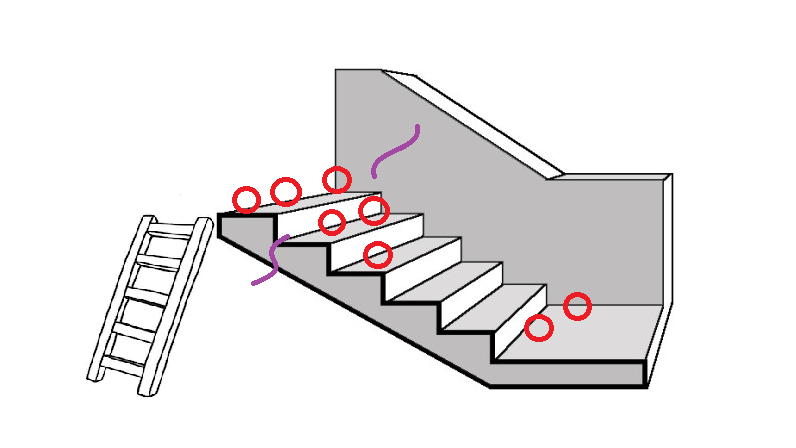
\includegraphics[scale=1.0]{Images2/Escalier 1.png}
    \caption{Un joli petit escalier et une jolie petite échelle}
    \label{fig:Analogie}
\end{figure}
On a choisi pour ce laser le néon et l'hélium, car le premier niveau d'excitation du second correspond très bien avec un état de haute énergie du second, la longueur de l'échelle correspond à une marche précise et haute de l'escalier en somme.\\
\begin{figure}[htp]
    \centering
    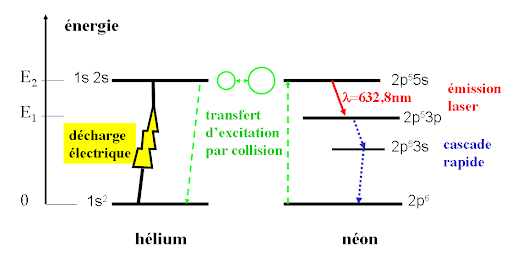
\includegraphics[scale=0.8]{Images2/hélium-néon.png}
    \caption{Schéma du fonctionnement du laser}
    \label{fig:schema_helium-neon}
\end{figure}



\newpage
\section{Transitions dipolaires}
\subsection{Expression du taux de transition}



Selon la théorie des perturbations dépendantes du temps au premier ordre\footnote{Voir le cours de MQ2 donné par Christophe Ringeval}, pour un système hydrogénoïde, le taux de transition $W$ (nous considérons un cas générique que nous appliquerons après à nos taux de transition $A_{21}$, $B_{12}$ et $B_{21}$) d'un état a d'énergie $E_a$ vers un état b d'énergie $E_b$ par absorption ou émission d'un photon de fréquence angulaire $w=|E_b-E_a|$ et sous une intensité $I$ est

\begin{equation}
    W\eq \dfrac{4\pi^2 \alpha \hbar}{m^2 w^2}I|M_{ba}|^2
\end{equation}
où $M_{ba}$ est l'élément de matrice de transition
\begin{equation}
    M_{ba}\eq \bra{\Psi_b}e^{-\imag\vec{k}\Cdot \vec{r}}\hat{\epsilon}\cdot\nabla \ket{\Psi_a}
    \label{Mba}
\end{equation}
où

\begin{itemize}[label=$\bullet$]
    \item $\vec{k}$ est le vecteur de propagation de l'onde
    \item $\hat{\epsilon}$ est le vecteur de polarisation
\end{itemize}
On peut tronquer le développement de Taylor de l'exponentielle
\begin{equation}
    e^{-\imag\vec{k}\Cdot\vec{r}}\eq 1-\imag\vec{k}\Cdot\vec{r}+\dfrac{1}{2!}(\imag\vec{k}\Cdot\vec{r})^2+...
    \label{eq:dvpl_expo}
\end{equation}
Si on garde seulement le premier terme de ce développement, on effectue ce qu'on appelle l'approximation dipolaire (physiquement, on néglige en fait les <<effets de retard>> à l'échelle de l'atome : si le photon a une longueur d'onde nettement supérieure à la taille de l'atome, tous les électrons de l'atome ressentiront le même champ E) et dans ce cas \eqref{Mba}, qu'on définit comme <<le moment dipolaire dans la représentation de vitesse>> devient
\[
    M_{ba} \;\simeq\; \bra{\Psi_b}\hat{\epsilon}\Cdot\nabla\ket{\Psi_a}
\]
De plus, on a que
\[
    m\vec{v}\eq \vec{p}\eq -\imag\hbar \nabla
\]
Donc
\[
    M_{ba} \simeq \dfrac{\imag m}{\hbar}\hat{\epsilon}\Cdot\bra{\Psi_b}\vec{v}\ket{\Psi_a}
\]
On sait aussi\footnote{Ceci vient directement de l'évolution de la valeur moyenne d'un opérateur au cours du temps : $\fdif{}{t}\langle A \rangle \eq \dfrac{1}{\imag\hbar}\langle[A,H] \rangle$} que $\vec{v}=\dot{r}=\dfrac{1}{\imag\hbar}[\vec{r},H_0]$ ce qui nous amène au moment dipolaire dans la représentation de longueur
\begin{align*}
    \bra{\Psi_b}\dot{\vec{r}}\ket{\Psi_a}
    &\eq
    \dfrac{1}{\imag\hbar}\bra{\Psi_b}\vec{r}H_0-H_0\vec{r}\ket{\Psi_a}\\
    &\eq
    \dfrac{1}{\imag\hbar}(E_a-E_b)\bra{\Psi_b}\vec{r}\ket{\Psi_a}\\
    &\eq
    \dfrac{1}{\imag\hbar}(-\hbar \omega)\bra{\Psi_b}\vec{r}\ket{\Psi_a} \\
    &\eq
    i \omega \bra{\Psi_b}\vec{r}\ket{\Psi_a} \\[5pt]
    \Longrightarrow \quad M_{ba} &\;\simeq\;
    -\dfrac{m \omega}{\hbar}\hat{\epsilon}\Cdot\bra{\Psi_b}\vec{r}\ket{\Psi_a}
\end{align*}
En remplaçant cette dernière expression de $M_{ba}$ dans l'expression du \textbf{taux de transition} $W$, on a
\[
    W\eq \dfrac{4\pi^2 \alpha}{\hbar}I |\hat{\epsilon}\Cdot\vec{r}_{ba}|^2
\]
On peut encore simplifier l'expression du taux de transition générique en prenant se valeur moyenne:
\[
    \int_{0}^{\pi/2} |\hat{\epsilon}\Cdot\vec{r}_{ba}|^2\sin{\theta} \dif\theta\eq |r_{ba}|^2\int_{0}^{\pi/2}\cos{\theta}^2\sin{\theta}\dif\theta\eq \dfrac{1}{3}|r_{ba}|^2
\]
Ainsi
\begin{equation}
    \overline{W}_{ba}\eq \dfrac{4\pi^2 \alpha}{3 \hbar}I |r_{ba}|^2
\end{equation}



    \subsection{Coefficients d'Einstein}



Les transitions radiatives sont caractérisées par les <<coeffients d'Einstein>>, qui décrivent les taux de transition par émission spontanée $A_{2\Rightarrow1}$, émission stimulée $B_{2\Rightarrow 1}$ et absorption $B_{1\Rightarrow2}$.\\
Conformément aux équations \eqref{eq:equilire1} et \eqref{eq:equilire1}, ces coefficients sont donnés par

\begin{equation}
    B_{ba}\eq \dfrac{\overline{W}_{ba}}{\rho}\eq \dfrac{c\overline{W}_{ba}}{I}\eq \dfrac{4\pi^2 c \alpha}{3 \hbar}|r_{ba}|^2
\end{equation}

\begin{equation}
    A_{ba}\eq \dfrac{\hbar w^3}{\pi^2 c^3}B_{ba}\eq \dfrac{4 \alpha}{3 c^2}w_{ba}^3|r_{ba}|^2
\end{equation}





\subsection{Cas d'un atome à $N$ électrons}

Dans le cas d'un atome à $N$ électrons, le terme d'interaction radiative s'écrit :

\subsection{Cas d'un atome à $n$ électrons}
Dans le cas d'un atome à $n$ électrons, le terme d'interaction radiative s'écrit :
\begin{equation}
    H_\text{rad}(t)\eq -\dfrac{\imag\hbar e}{m}\sum_{i=1}^{N} \vec{A}(\vec{r}_i,t).\nabla_i
\end{equation}
En unités atomiques, l'élément de matrice de transition dipolaire en représentation de longueur est ($\hat{\bm{\epsilon}}$ est, pour rappel, un vecteur) :
\begin{equation}
    M_{ba} \eq
    -\omega \hat{\bm{\epsilon}}\cdot\bra{\Psi_b}\sum_{i=1}^{N} \bm{r}_i\ket{\Psi_a}
    \eq
    -\omega \bra{\Psi_b}\hat{\bm{\epsilon}} \cdot \bm{D}\ket{\Psi_a}
    \eq
    -\omega \sum_{q=0,\pm 1}\bra{\Psi_b}\hat{\epsilon}_q^* D_q\ket{\Psi_a}
\end{equation}
où nous avons défini le vecteur $\bm{D}$, avec $i$ l'indice dénotant l'électron :
\[
    \bm{D} \;\equiv\; \sum_{i=1}^N \bm{r}_i
\]
et utilisé la définition du produit scalaire:
\begin{equation}
    \hat{\bm{\epsilon}}\Cdot \bm{r} \eq \hat{\epsilon}_xx + \hat{\epsilon}_yy + \hat{\epsilon}_zz \eq \sum_{q=0,\pm 1}  \hat{\epsilon}_q^* r_q
\end{equation}
L'opérateur $\bm{D}$ est un opérateur vectoriel, c'est-à-dire un opérateur tensoriel irréductible de rang 1. La généralisation des règles de sélection découle du théorème de Wigner-Eckart (qui, apparemment, découle de la théorie des groupes et qui est vachement long à démontrer donc on le prend comme acquis et on ne cherche pas vraiment à le comprendre) :
\begin{equation}
    \bra{\tau ` J'M'}D_q\ket{\tau JM}\eq \dfrac{1}{\sqrt{2J'+1}}\bra{\tau `J'}|\vec{D}|\ket{\tau J}\bra{J1Mq}\ket{J'M'}
\end{equation}
Les coefficients de Clebsch-Gordan sont donc nuls sauf si

\[
    J'\eq |J-1|, |J-1|+1, ..., J+1
\]

\[
    M+q\eq M'
\]

On a donc les règles de sélection pour une transition dipolaire électrique (E1):

\begin{equation}
    \Delta J\eq 0, \pm1 \quad \text{et} \quad \Delta M\eq 0, \pm 1 \quad \text{et        changement de parité}
\end{equation}



De façon tout à fait équivalente, mais en considérant le terme en $\vec{k}\Cdot\vec{r}$ dans l'équation \eqref{eq:dvpl_expo}, nous pouvons trouver les règles de sélection pour les transitions interdites. Tout ceci est fait dans le syllabus du Pr Terao-Dunseath.


\begin{figure}[htp]
    \centering
    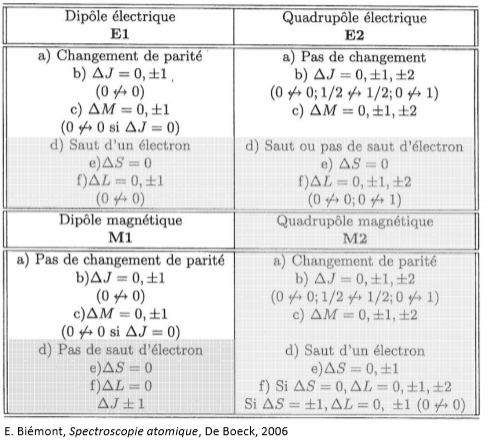
\includegraphics[scale=0.8]{Images2/regles.PNG}
    \caption{Règles de sélection des transitions radiatives}
    \label{fig:regles_transision_radiatives}
\end{figure}

\subsection{Diagramme de Grotrian}
Un diagramme de Grotrian (Fig. \ref{fig:grotrian}) indique les transitions permises entre les niveaux d'énergie des atomes. Il tient compte des règles de sélection liées aux changements de moment cinétique orbital et de spin des électrons.

Un diagramme de Grotrian indique les transitions permises entre les niveaux d'énergie des atomes. Il tient compte des règles de sélection liées aux changements de moment cinétique orbital et de spin des électrons.

\begin{figure}[htp]
    \centering
    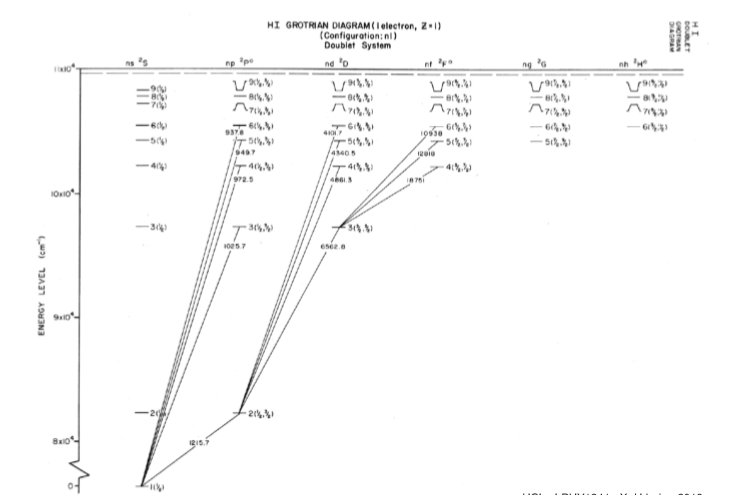
\includegraphics[width=0.7\textwidth]{Images2/grotrian.PNG}
    \caption{Exemple de diagramme de Grotrian}
    \label{fig:grotrian}
\end{figure}



%-------------------- 2e Partie Urbain ----------------------
\newpage
\section{Hamiltonien spin-orbite et hyperfin}
\subsection{Hamiltonien spin-orbite}


L'électron possède un spin et un moment cinétique orbital. Nous avons donc une charge en mouvement, ce qui provoque un moment magnétique orbital. Ces deux moments magnétiques (de spin et orbital) interagissent ensemble et cette interaction est décrite pas l'hamiltonien de spin-orbite\footnote{D'où le <<SO>> du $W_\text{SO}$}, qui peut être traité comme une perturbation de l'hamiltonien $H_0$. L'hamiltonien associé à l'interaction du moment magnétique de spin avec le champ magnétique de l’électron en mouvement s'écrit

\[
    W_\text{SO} \eq  -\vec{\mu_\text{s}}\Cdot\vec{B}'
\]

avec $-\vec{\mu_\text{s}}$ le moment magnétique de spin. On rappelle les quantités suivantes:

\begin{enumerate}
    \item Moment magnétique créé par une boucle de courant :
    \[
        \vec{\mu} \eq \vec{I}\cross \vec{A} \eq -\dfrac{e\vec{v}}{2\pi r}\cross \pi r^2\hat{r} \eq -\dfrac{e}{2m}\vec{l}
    \]
    Attention : $\hat{r}$ désigne le vecteur $\dfrac{\vec{r}}{\abs{\vec{r}}}$ sa norme est donc égale à 1, $\vec{A}$ désigne le vecteur radial dont la norme représente la surface de la boucle de courant. On part de l'expression classique $\vec{\mu} = i\vec{S}$ où l'intensité $i = \dfrac{e|\vec{v}|}{2\pi r}$ et $S = \pi r^2$. Pour avoir un vecteur $\vec{S}$ perpendiculaire à la surface, on prend le produit vectoriel de $\vec{r}$ et $\vec{v}$. $\vec{l}$ est le vecteur moment orbital et s'écrit $m\vec{v}\cross\vec{r}$.
    \item Magnéton de Bohr et son implication pour le moment magnétique créé par une boucle de courant :
    \[
        \mu_\text{B} \eq \dfrac{e\hbar}{2m} \quad \Leftrightarrow \quad \vec{\mu} \eq -\mu_\text{B}\dfrac{\vec{l}}{\hbar}
    \]
    \item Par analogie à l'expression du moment magnétique créé par une boucle de courant (point au-dessus), nous pouvons écrire le moment magnétique de spin comme:
    \[
        \vec{\mu_\text{s}} \eq -g\mu_\text{B}\dfrac{\vec{s}}{\hbar} \qquad \textrm{avec } g=2.
    \]
    où nous avons utilisé le rapport gyromagnétique $g$, qui est défini comme étant \emph{le rapport entre le moment magnétique  et le moment cinétique d'une particule}.
    % utile le truc avec les unités?
    Pour mieux comprendre ce qu'on fait, on peut raisonner sur les unités : $\vec{\mu} = [\si{m^2kg/s}] = [\si{Js}]$. $\hbar$ a donc les unités d'un moment angulaire.
    \item Champ magnétique :
    \[
        \vec{B}' \eq \dfrac{\vec{B} - \vec{v}\cross \dfrac{\vec{E}}{c^2}}{\sqrt{1-\dfrac{v^2}{c^2}}} \simeq -\dfrac{\vec{v}\cross \vec{E}}{c^2}
    \]
    On ignore donc ici le boost de Lorentz lié à la correction relativiste.
    \item Champ électrique :
    \[
        \vec{E} \eq  -\dfrac{1}{e}\dfrac{\partial U}{\partial r}\hat{r}
    \]
\end{enumerate}

On peut donc réécrire l'interaction $W_\text{SO}$ comme suit,

\begin{equation}
    W_\text{SO} \eq  \dfrac{1}{2m^2c^2}\dfrac{1}{r}\dfrac{\partial U}{\partial r}(\vec{l}\Cdot\vec{s}) \eq  \zeta(r)\vec{l}\Cdot\vec{s}
    \quad\Longrightarrow\quad
    W_\text{SO}^{tot} \eq \sum_i\zeta(r_i)\vec{l_i}\Cdot\vec{s_i}
    \label{eq:Hamilt_SO}
\end{equation}

avec $\vec{l}$ le moment angulaire et $\sum_i...$ la somme sur les opérateurs mono électroniques. Il y a différentes façons de dériver l’hamiltonien spin-orbite : on peut partir de l’équation de Dirac\footnote{Il s'agit d'une équation de Schrödinger relativiste pour les fermions, donc les électrons} ou alors traiter l’hamiltonien spin-orbite comme étant l’interaction du moment de spin, qu’on définit par analogie avec le moment magnétique d’une boucle de courant pour autant qu’on introduise le rapport gyromagnétique ($g$) à peu près égal à 2. À côté de ça, on a un champ magnétique $B$ qui est essentiellement causé par la présence d’un champ électrique dans le voisinage du noyau. Ce champ électrique pointe dans la direction radiale si on a un potentiel à symétrie centrale.\footnote{Ou alors on peut utiliser le raisonnement fait en quantique 2 en disant que c'est le proton qui tourne autour de l'électron et que le spin de l'électron interagit avec le champ magnétique créé par le noyau.}\\

Pour chaque électron, cette interaction spin-orbite est proportionnelle au produit scalaire du moment angulaire de cet électron et du spin de ce même électron (l'interaction spin-orbite concerne un électron et son propre moment angulaire). La fonction $\zeta(r)$ cache un peu tout ce qui va dépendre de la distance électron-noyau. Le facteur en $\dfrac{1}{r}$ implique que ce potentiel agit essentiellement au voisinage du noyau : l'interaction SO se passera donc surtout proche du noyau. Quand on a plusieurs électrons, on va faire une somme.

Nous allons maintenant effectuer une approximation de l'expression \eqref{eq:Hamilt_SO} : nous allons remplacer la somme d’opérateurs mono électroniques par le produit scalaire du moment angulaire total et du spin total. Étant donné que nous devons travailler en termes de $\vec{J}$ et non en termes de $\vec{L}$ ou $\vec{S}$, on va travailler avec des états de $\vec{J}$ total défini (pas de $\vec{L}$ ou de $\vec{S}$ défini). On peut donc passer d’une base à l’autre en réécrivant l’opérateur $\vec{L}\Cdot\vec{S}$.

\begin{equation}
    \vec{L}\Cdot\vec{S} \eq  \dfrac{1}{2}(J^2-L^2-S^2) \qquad \mathrm{avec} \quad \vec{J} \eq  \vec{L}+\vec{S}
    \label{eq:JLS}
\end{equation}
On se retrouve avec un élément de matrice de la forme donnée à l'équation \eqref{eq:Hamilt_SO_J1} où nous avons introduit un préfacteur $A(\gamma L S)$\footnote{Le $gamma$ représente les autres nombres quantiques, si jamais on a un ECOC avec plus d'observables} qui cache la structure atomique, mais qui est supposé représenter le facteur $\zeta(r_i)$. Nous avons donc une expression ne faisant plus intervenir que le moment angulaire total et non plus sur le moment angulaire de chaque électron.

\begin{align}
    \langle \gamma LSM_LM_S|H_\text{SO}|\gamma LSM_L'M_S' \rangle &\eq  A(\gamma LS)\langle \gamma LSM_LM_S|\vec{L}\Cdot\vec{S}|\gamma LSM_L'M_S' \rangle
    \label{eq:Hamilt_SO_J1}    \\
    &\eq
    \dfrac{1}{2}A(\gamma LS)\left( J(J+1)-L(L+1)-S(S+1)\right)
    \label{eq:Hamilt_SO_J2}
\end{align}
La formule \eqref{eq:JLS} nous permet d’écrire l'équation \eqref{eq:Hamilt_SO_J2}, et cette formulation nous permet d'établir la règle de Landé (cf. figure \ref{fig:RegleLandé} où la colonne des $J$ est celle des états de structure fine) : pour une même valeur de $L$ et de $S$, l’écart en énergie entre le niveau $J$ et le niveau $J-1$ est proportionnel à $J$.

\begin{figure}[htp]
    \centering
    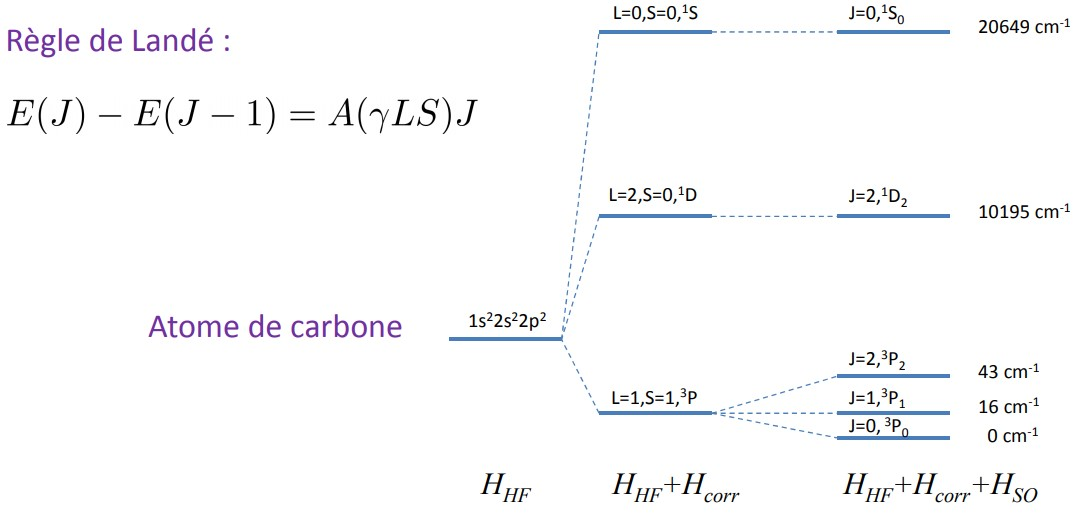
\includegraphics[scale=0.50]{Images2/regleLande.jpg}
    \caption{Règle de Landé.}
    \label{fig:RegleLandé}
\end{figure}

Donc il y a une première opération qui consiste à chercher les termes et vérifier que le terme de plus basse énergie est celui de multiplicité de spin la plus grande (règle de Hund). Ensuite, il faut encore coupler $\vec{L}$ avec $\vec{S}$ (pour obtenir $\vec{J}$) et pour un même couple $(L,S)$, on a les états de structure fine avec la correction de spin-orbite, sur lesquels on peut appliquer la règle de Landé.

En réalité, il existe d'autres corrections comme la monoconfiguration ou la correction au fait que nous avons considéré le moment angulaire total et le spin total au lieu des moments angulaires et de spin individuels (remplacement de la somme d'opérateurs monoélectroniques de l'équation \eqref{eq:Hamilt_SO}). Notre approximation a donc un impact sur la précision de la formule de Landé.

Mais on n’en a pas fini, il y a aussi la structure hyperfine! Nous avons donc pris en compte la correction de spin-orbite (couplage du moment magnétique de spin avec le moment magnétique orbital). Il nous reste à tenir compte de \textbf{l’interaction du spin du noyau, avec d'une part le spin des électrons, et d'autre part leur moment angulaire.}



\subsection{Hamiltonien hyperfin}

Nous allons ici considérer l'interaction du spin nucléaire, noté $\vec{I}$, avec d'une part le spin des électrons et d'autre part le moment magnétique des électrons. Pour commencer, et par analogie avec le moment magnétique de spin des électrons, notons le moment magnétique de spin du noyau (que nous couplerons après) :

\begin{equation}
    \vec{\mu_\text{I}}
    \eq -g_\text{I}\mu_\text{N}\dfrac{\vec{I}}{\hbar}
    \eq  g_\text{I}'\mu_\text{B}\dfrac{\vec{I}}{\hbar}
    \label{eq:momt_magn_nucl}
\end{equation}
avec $g_\text{I}$ le rapport gyromagnétique, $\mu_\text{N}$ le magnéton nucléaire, $\mu_\text{B}$ le magnéton de Bohr et $g_\text{I}'=\dfrac{m_e}{M_\text{N}}g_\text{I}$. Nous avons ici réintroduit le magnéton de Bohr en faisant apparaître le rapport de la masse de l’électron sur celle du noyau. Ce rapport étant très petit, le moment magnétique nucléaire est beaucoup plus petit que le moment magnétique électronique.

Pour exprimer le champ magnétique (créé par le moment orbital des électrons), on repart de la loi (classique $\longrightarrow$ approximation !) de Biot-Savart : la circulation des électrons génère un champ magnétique à la position du noyau.
\begin{equation}
    \vec{B}' \eq
    -\dfrac{\mu_0}{4\pi}e\dfrac{\vec{r}}{r^3}\cross \vec{v} \eq
    -\dfrac{\mu_0}{2\p\imag\hbar}\dfrac{\vec{l}}{r^3}
    \label{eq:champ_B}
\end{equation}
En combinant les résultats des équations \eqref{eq:momt_magn_nucl} et \eqref{eq:champ_B}, c'est-à-dire en couplant le moment magnétique nucléaire avec le champ magnétique, nous obtenons la contribution hyperfine du spin du noyau à l'hamiltonien :

\[
    W_\text{hyp} \eq
    - \vec{\mu_I} \Cdot \vec{B}'
    \eq
    \dfrac{\mu_0}{2\p\imag\hbar^2} g_\text{I} \mu_\text{N} \mu_\text{B} \dfrac{\vec{l}\Cdot\vec{I}}{r^3}
\]
On rajoute maintenant les termes d'interactions entre spins nucléaire et électronique et on obtient

\begin{equation}
    W_\text{hyp} \eq  \dfrac{\mu_0}{2\p\imag\hbar^2}g_\text{I}\mu_\text{N}\mu_\text{B}\dfrac{1}{r^3}\left( \vec{l}\Cdot\vec{I}-\vec{s}\Cdot\vec{I} + 3(\vec{s}\Cdot\hat{r})(\vec{I}\Cdot\hat{r}) \right).
\end{equation}
Le premier produit scalaire correspond à l'interaction entre le champ magnétique induit par déplacement du noyau dans le champ électrique créé par l'électron. Il s'agit donc de la situation analogue à l'interaction spin-orbite pour le noyau. Les deux autres termes représentent l'interaction du spin orbital avec le spin nucléaire, de l'alignement de leurs boussoles. La forme a été dérivée explicitement dans le cours de Mécanique Quantique 2.\\
En posant $\vec{G} = \vec{L} - \vec{S} + 3(\vec{S}\Cdot\hat{r}) \hat{r}$, l'hamiltonien hyperfin devient :

\begin{equation}
    W_\text{hyp} \eq  \dfrac{\mu_0}{2\p\imag\hbar^2}g_\text{I}\mu_\text{N}\mu_\text{B}\langle\dfrac{1}{r^3}\rangle \vec{G}\Cdot\vec{I}.
\end{equation}
Pour avoir l’énergie d’interaction résultant de la prise en compte du spin nucléaire, il nous faut évaluer le produit scalaire $\vec{G} \Cdot \vec{I}$. Ce produit scalaire n’est pas sous une forme que nous pouvons utiliser, mais nous allons le réécrire via le théorème de Wigner-Eckart. On notera que lorsqu’on a un opérateur vectoriel $\vec{K}$, ses éléments de matrice peuvent toujours se réexprimer comme des éléments de matrice du moment cinétique $\vec{J}$.



\subsubsection{Théorème de Wigner-Eckart (corollaire)}

Soit $K_q$ la q$^\text{ème}$ composante standard d'un opérateur vectoriel $\vec{K}$ et $J_q$ celle du moment cinétique $\vec{J}$. Soient $|\tau JM\rangle$, $|\tau JM'\rangle$ deux vecteurs appartenant au même sous-espace. Alors,

\[
    \langle\tau JM|K_q|\tau JM'\rangle \eq   \langle\tau JM|J_q|\tau JM'\rangle\dfrac{ \langle\tau JM|\vec{J}\Cdot\vec{K}|\tau JM'\rangle}{J(J+1)}.
\]
De plus,

\[
    \langle |\vec{G}\Cdot\vec{I}| \rangle \eq  \dfrac{\langle |\vec{G}\Cdot\vec{J}| \rangle\langle |\vec{J}\Cdot\vec{I}| \rangle}{\hbar^2J(J+1)}
\]
\textbf{Démonstration :}
\[
    \bra{b}\vec{G}\ket{a}
    \eq c\bra{b}\vec{J}\ket{a}
\]
\begin{align*}
    \bra{b}\vec{G} \Cdot \vec{J}\ket{a}
    &\eq  c\sum_k \bra{b}\vec{J}\ket{k}\bra{k}\vec{J}\ket{a}\\
    &\eq  c\bra{b}J^2\ket{a}\\
    &\eq  c\hbar^2 J(J+1)
\end{align*}
\[
    \bra{b}\vec{G}\ket{a} \eq \dfrac{\bra{b}\vec{G} \Cdot \vec{J}\ket{a}}{\hbar^2 J(J+1)}\bra{b}\vec{J}\ket{a}
\]
On a donc :

\[
    \langle |\vec{G}\Cdot\vec{I}| \rangle \eq  \dfrac{\langle |\vec{G}\Cdot\vec{J}| \rangle\langle |\vec{J}\Cdot\vec{I}| \rangle}{\hbar^2J(J+1)}
\]
et \footnote{\text{On obtient $(\vec{S}\Cdot\hat{r})^2 = \dfrac{S^2}{3}$ par isotropie de la norme de l'opérateur vectoriel.}}

\begin{align*}
    \vec{G}\Cdot\vec{J}
    &\eq  (\vec{L}-\vec{S}+3(\vec{S}\Cdot\hat{r})\hat{r}).(\vec{L}+\vec{S})\\
    &\eq L^2 + \vec{L}\Cdot\vec{S} -\vec{L}\Cdot\vec{S} - S^2 + 3 (\vec{S}\Cdot\hat{r})\underbrace{(\vec{L}\Cdot\hat{r})}_{= 0} + +\underbrace{3(\vec{S}\Cdot\hat{r})^2}_{=S^2}\\
    &\eq  L^2
\end{align*}
Utilisant ces résultats, notre terme de correction hyperfine devient :

\begin{equation}
    W_\text{hyp} \eq  \dfrac{\mu_0}{2\p\imag\hbar^2}g_\text{I}\mu_\text{N}\mu_\text{B}\langle\dfrac{1}{r^3}\rangle \dfrac{L^2}{J^2}\vec{J}\Cdot\vec{I}.
\end{equation}
Cette correction fait intervenir tous les états de même $J$. On définit un nouvel opérateur $\vec{F}$ tel que $\vec{F} = \vec{I} + \vec{J}$. Dès lors, puisque $\vec{J}\Cdot\vec{I} \eq  \dfrac{1}{2}(F^2-I^2-J^2)$, la correction hyperfine  de l'énergie devient (la démonstration de ce théorème n'est pas reprise ici):

\begin{align*}
    \Delta E_\text{hyp} &\eq  \dfrac{\mu_0}{2\p\imag\hbar^2}g_\text{I}\mu_\text{N}\mu_\text{B}\langle\dfrac{1}{r^3}\rangle\dfrac{L(L+1)}{J(J+1)}\left( F(F+1) - J(J+1) - I(I+1) \right)\\
    &\;\equiv\;
    \dfrac{C}{2} \left( F(F+1) - J(J+1) - I(I+1) \right)
\end{align*}
(Bien que ce soit repris tel quel dans les slides, nous avons un doute quant à l'absorption du facteur $\dfrac{L(L+1)}{J(J+1)}$ par la constante $C$).

En prenant maintenant toutes les corrections que nous avons faites à $H_\text{HF}=H_\text{Hartree-Fock}$ (c'est-à-dire $H_\text{corr}$\footnote{Corrections dues aux différents termes}, $H_\text{SO}$ et $H_\text{Hyperfin}$), nous obtenons à la figure \ref{fig:regle_lande2} une généralisation de la figure \ref{fig:RegleLandé} pour un atome de Na ($I=\dfrac{3}{2}$). Nous obtenons ainsi la généralisation de la règle de Landé qui inclut la correction hyperfine : la différence entre deux niveaux consécutifs (en termes de $F$) de même $L$, $S$ et $I$ est proportionnel à $F$.
En outre, on remarque que le nombre de niveaux hyperfins va augmenter au fur et à mesure qu'on va monter en moment angulaire total $J$.
\begin{figure}[htp]
    \centering
    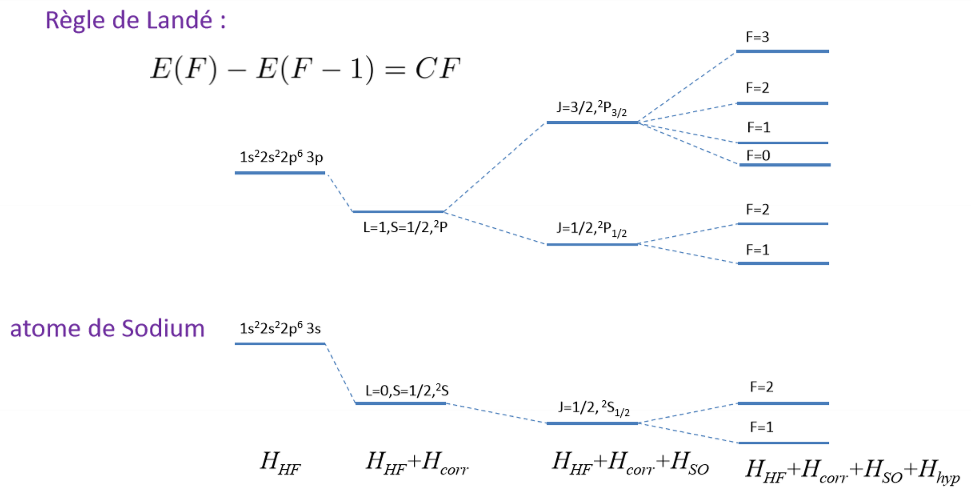
\includegraphics[scale=0.8]{Images2/règle_Landé2.png}
    \caption{Règle de Landé dans le cas d'une correction hyperfine. Pour le Na, $I=\dfrac{3}{2}$}
    \label{fig:regle_lande2}
\end{figure}


Nous venons donc de traiter d'une correction hyperfine, celle traitant du spin du noyau. Pour le fun, nous pouvons également calculer la correction hyperfine liée à la non-sphéricité du noyau grâce à l'opérateur $\vec{K}$. Ce calcul est fort compliqué (selon les dires du professeur) et c'est pourquoi nous ne présentons que le résultat (Fig. \ref{fig:eq_correcK}), en se rappelant que $\vec{F} \eq \vec{J} \; + \; \vec{I}$.
\begin{figure}[htp]
    \centering
    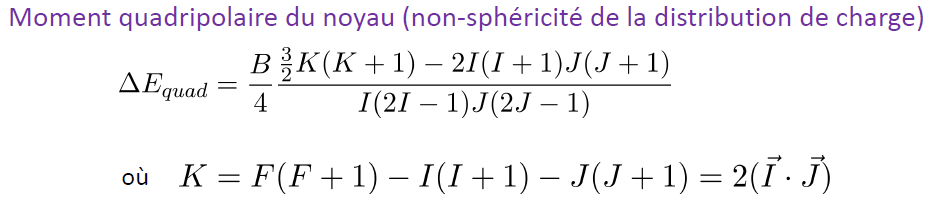
\includegraphics[scale=0.80]{Images2/CorrecK.PNG}
    \caption{Correction de non-sphéricité}
    \label{fig:eq_correcK}
\end{figure}
En résumé, nous avons la correction énergétique suivante (Fig. \ref{fig:eq_resume_correct}), en tenant compte du couplage spin-orbite, du spin du noyau et de la non-sphéricité du noyau:
\begin{figure}[htp]
    \centering
    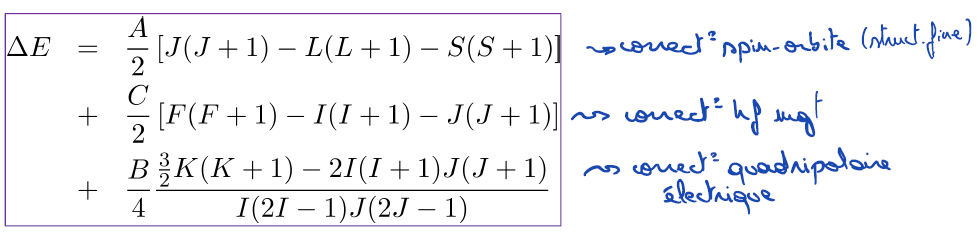
\includegraphics[scale=0.80]{Images2/résuméCorrec.PNG}
    \caption{Résumé des corrections hyperfines}
    \label{fig:eq_resume_correct}
\end{figure}
où A,B et C sont des constantes déterminées pour chaque atome décrivant ces interactions.


\newpage
\subsection{Applications expérimentales}
\subsubsection{Différencier deux isotopes}



Dans le cas de deux isotopes d'un même élément, on va observer deux graphes identiques jusqu'à la correction hyperfine de volume nucléaire. Là, on observera deux spins nucléaires différents qui permettront de déterminer l'isotope observé.\footnote{Rappel : le neutron est un fermion de spin $\dfrac{1}{2}$.} Prenons deux isotopes de l'atome de Rubidium par exemple :
\begin{figure}[htp]
    \centering
    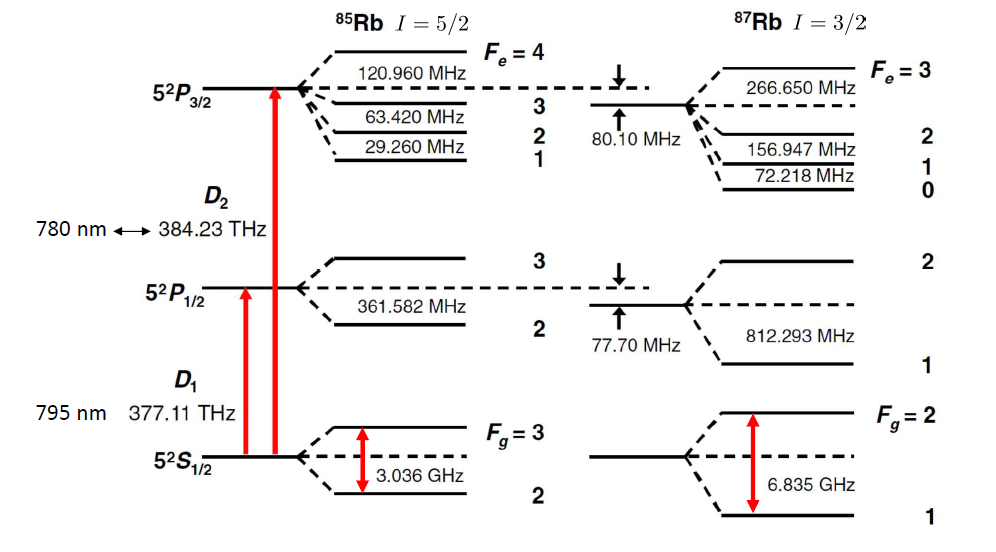
\includegraphics[scale=0.8]{Images2/ComparaisonRb.PNG}
    \caption{Structure hyperfine du $^{87}Rb$ et du $^{85}Rb$}
\label{eq:struct_hyperfine}
\end{figure}
On remarque tout de suite que la correction hyperfine de non-sphéricité se distingue beaucoup plus pour les niveaux de basse énergie que pour les niveaux de haute énergie (le graphe n'est pas à l'échelle). En effet, cette correction hyperfine n'est, à basse énergie, pas <<gommée>> par des corrections fines. On remarque également que la règle de Landé est satisfaite.\\
Sachant que le Rb est un métal alcalin (sa structure électronique est celle d'un gaz rare + un électron), nous savons que $S = \dfrac{1}{2}$ et, par conséquent, nous pouvons identifier $I = \dfrac{3}{2}$ pour $^{87}$Rb et $I = \dfrac{5}{2}$ pour $^{85}$Rb. Il s'agit du critère qui nous permet de différencier les isotopes.



\subsubsection{Spectroscopie par absorption}


Nous souhaitons observer expérimentalement toutes ces transitions, dont les fréquences ont un même ordre de grandeur. Un schéma expérimental possible pour observer ces transitions est donné à la figure \ref{fig:SchemaAbso}.
\begin{figure}[htp]
    \centering
    \includegraphics[scale=1.0]{Images2/SchémaAbso.PNG}
    \caption{Schéma d'une expérience par absorption}
    \label{fig:SchemaAbso}
\end{figure}
De la lumière est émise dans un spectre contrôlé de fréquence sur un échantillon d'atomes selon l'axe z. Une partie de l'intensité émise est absorbée par des phénomènes de résonance avec les niveaux d'énergie des atomes du milieu. On a donc en sortie de l'expérience un graphe d'absorption (avec des bosses) on de transmission (avec des creux).\\

Expérimentalement, le fait de ne pas travailler à température nulle entraîne des effets Doppler qui nous empêchent d'observer des pics bien définis aux fréquences de transition. Plus explicitement, seules les transitions concernant des atomes se déplaçant perpendiculairement à la direction z vont se faire à la fréquence définie. Les autres atomes subissent un redshift s'ils se déplacent vers la droite ou un blueshift s'ils se déplacent vers la gauche. On observe donc une gaussienne conformément à la distribution de Maxwell-Boltzmann. À noter que l'on peut donc extraire à partir de ce genre d'expérience la température du milieu (applications en astrophysique). On obtient en sortie ce genre de figure.\\

\begin{figure}[htp]
    \centering
    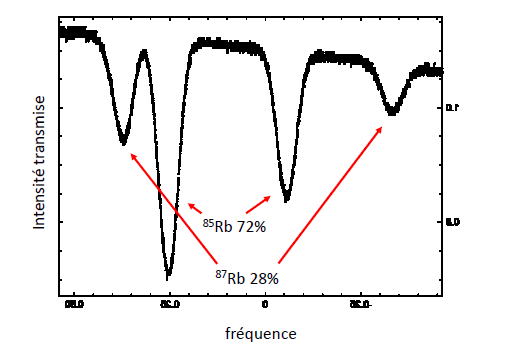
\includegraphics[scale=1.0]{Images2/Absorption.PNG}
    \caption{Figure de transmission pour deux isotopes du rubidium}
    \label{fig:abso}
\end{figure}

La montée générale en transmission en augmentant la fréquence (en allant vers la gauche donc, attention à l'axe) provient du comportement des diodes émettrices et n'est pas liée à un phénomène physique dans l'enceinte.

En plus de l'effet Doppler, il y a également une limitation fondamentale propre à la mécanique quantique qui nous empêche d'avoir des pics de largeur infinitésimale. Le temps de vie des états excités est typiquement assez faible, par le principe d'incertitude temps/énergie on a donc des ré-émissions dans une gamme d'énergie <<inexactes>>, et cela tout à fait indépendamment du dispositif expérimental. En mots profanes, dû au temps de vie très faible des atomes (très faible incertitude sur leur temps de vie), les atomes introduisent une part d'incertitude dans les fréquences qu'ils ré-émettent (gamme très large d'énergie) après désexcitation à cause du principe d'Heisenberg (pour le temps et l'énergie).\\

Sur la figure \ref{fig:abso}, on peut donc distinguer deux isotopes. Comme dit précédemment, la différence hyperfine de spectre entre les deux est induite par une modification du spin nucléaire par l'ajout de deux neutrons. L'intensité relative des pics (=hauteur/profondeur des gaussiennes) nous informe sur la composition isotopique du mélange. Attention cependant, dans ce genre d'expériences on surestime toujours largement la température de l'environnement, car la gaussienne est le produit de la superposition de plusieurs gaussiennes plus petites correspondant à des transitions entre états excités. Pour faire apparaître le détail de ces petites gaussiennes, on se sert de la spectroscopie pas absorption saturée.


\subsubsection{Spectroscopie par absorption saturée}
Avis au lecteur : cette partie s'inspire fortement de Wikipédia ; on a essayé de recouper l'article avec le cours.\\
\begin{figure}[htp]
    \centering
    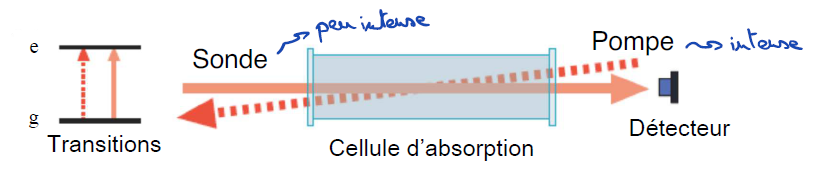
\includegraphics[width=\textwidth]{Images2/AbsoSatu.PNG}
    \caption{Schéma expérimental pour l'absorption saturée}
\label{fig:absoSatu}
\end{figure}
L'idée de ce montage expérimental est d'exploiter notre contrôle sur la direction de propagation de la lumière. On va superposer deux faisceaux de même fréquence : d'une part nous aurons un faisceau \textbf{sonde} (\textit{probe}) de faible intensité allant dans la direction $+z$ et d'autre part nous aurons un faisceau \textbf{pompe} (\textit{pump}) de forte intensité allant dans la direction $-z$. On note également que ce qui est observé dans le détecteur est le résultat de la propagation du faisceau <<sonde>> dans l'environnement ; le faisceau pompe n'a aucune incidence directe sur notre détecteur.

Supposons que la fréquence des faisceaux soit légèrement désaccordée vers le rouge par rapport à la fréquence propre des atomes. Alors le faisceau pompe va interagir avec les atomes dont la vitesse suivant l'axe $z$ sera positive, qui se rapprochent de la source de photons ; ainsi grâce à l'effet Doppler le faisceau pompe est à la bonne fréquence pour ces atomes. Le faisceau sonde, lui va interagir avec d'autres atomes, à savoir ceux dont la vitesse suivant l'axe $z$ est négative. Un même raisonnement peut être tenu pour une fréquence légèrement décalée vers le bleu. Ce comportement est représenté à la figure \ref{fig:vit2}. Attention il ne s'agit pas d'un motif que l'on retrouve expérimentalement (car les vitesses étant isotropes, les effets symétriques se compensent).

\begin{figure}[htp]
    \centering
    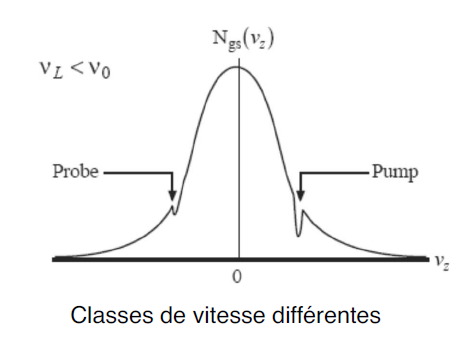
\includegraphics[scale=1.0]{Images2/Vitesse2.PNG}
    \caption{Figure d'absorption pour des classes de vitesse différentes}
\label{fig:vit2}
\end{figure}

Si maintenant les faisceaux sont exactement à la fréquence propre des atomes, alors les faisceaux pompe et sonde interagissent avec les mêmes atomes, ceux dont la vitesse suivant l'axe $z$ est nulle (pas besoin d'effet Doppler pour être résonnant). Comme le faisceau pompe est intense, il sature la transition atomique, ce qui signifie qu'un photon issu de la sonde arrivant sur un atome dont la vitesse selon $z$ est nulle a une forte probabilité de trouver l'atome dans son état excité. L'interaction entre le photon et l'atome n'est alors pas une absorption, mais correspond au phénomène d'émission stimulée, et a pour conséquence que le photon issu de la sonde continue son chemin et fini par sortir de l'échantillon : le faisceau sonde est beaucoup moins absorbé qu'en l'absence du faisceau pompe (ce qui correspondrait à une spectroscopie classique). En regroupant les résultats du détecteur pour différentes fréquences des faisceaux sonde et pompe, on voit donc apparaître un profil gaussien dû à l'effet Doppler, et au milieu de ce profil un pic étroit qui correspond à une transmission à nouveau élevée : la position de ce pic correspond à la fréquence de transition de l'atome.

En pratique ces pics plus étroits permettent d'identifier des transitions hyperfines qui étaient cachées par la largeur de la gaussienne principale.
\begin{figure}[htp]
    \centering
    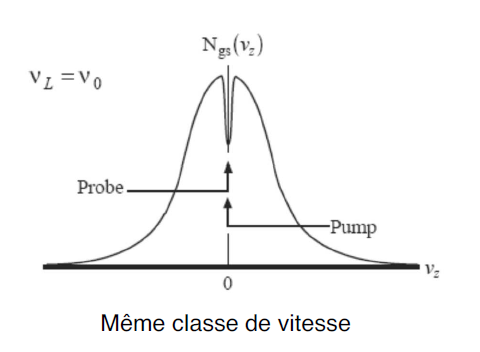
\includegraphics[scale=1.0]{Images2/Vitesse1.PNG}
    \caption{Figure d'absorption pour des classes de vitesse équivalentes}
\label{fig:vit1}
\end{figure}


%Les deux faisceaux se propageant dans des sens opposés, ils subissent les effets du décalage Doppler. C'est ce qui est illustré à la figure \ref{fig:vit2}. Attention il ne s'agit pas d'un motif que l'on retrouve expérimentalement (car les vitesse étant isotropes, les effets symétriques se compensent). Il permet néanmoins d'exprimer que pour une classe de vitesse particulière (non perpendiculaire à $x$), un ensemble d'atomes du gaz se déplaçant donc dans la même direction à la même vitesse, l'interaction avec le faisceau est symétriquement opposée. L'un subit un blueshift, l'autre un redshift.
%Cependant, lorsque la particule se déplace perpendiculairement à l'axe de propagation de la lumière elle interagit avec les faisceaux sonde et pompe (pas d'effet Doppler). On a donc une diminution de l'absorption par rapport au cas <<sonde seule>>. En effet, les atomes concernés, appartenant à la classe de vitesse perpendiculaire donc, ont déjà été excités par le faisceau pompe. On observe donc pour ces atomes une émission stimulée qui permet au photon qui la subit de continuer son chemin à la même fréquence entraînant donc cette chute caractéristique de l'absorption au centre de la gaussienne. Il s'agit du seul changement qu'on observe expérimentalement.\\
%En pratique ces pics plus étroits permettent d'identifier des transitions hyperfines qui étaient cachées par la largeur de la gaussienne principale.




\subsection{Effet Zeeman}



\textbf{Définition :} l'effet Zeeman décrit la levée de dégénérescence et plus généralement la modification des niveaux d'énergie d'un atome plongé dans un champ \textbf{magnétique} extérieur.\\
Il s'agit donc ici d'évaluer l'interaction entre la spire de courant que sont les électrons et le champ magnétique extérieur $\vec{B}$. On écrit donc l'Hamiltonien d'interaction ainsi que le moment magnétique total $\vec{\mu}$, avec
\begin{itemize}[label=$\bullet$]
    \item $\vec{\mu}_{s}$, le moment magnétique de spin
    \item $\vec{\mu}_{l}$, le moment magnétique orbital
    \item $\mu_\text{B}$, le magnéton de Bohr
    \item $g$, le rapport gyromagnétique tel que $g \approx 2$
\end{itemize}

\[
    H_B \eq -\vec{\mu} \Cdot \vec{B}
\]
\[
    \vec{\mu} \eq \vec{\mu}_{s} + \vec{\mu}_{l} \eq \sum_i \vec{\mu}_{s_i} + \vec{\mu}_{l_i} \; \approx \; \dfrac{\mu_\text{B}}{\hbar}\left( \vec{L} + g\vec{S}\right)
\]
On réécrit donc l'Hamiltonien d'interaction \emph{pour un champ $\vec{B}$ purement selon $z$} ainsi :

\[
    H_B \;\approx\; \dfrac{\mu_\text{B}}{\hbar}\left( L_z + 2 S_z\right)B_z \eq \dfrac{\mu_\text{B}}{\hbar}\left( J_z + S_z\right)B_z
\]
On applique de nouveau le théorème de Wigner-Eckart pour réexprimer l'élément de matrice de $\vec{S}$ comme le multiple de l'élément de $\vec{J}$.

\begin{equation}
    \bra{bJ}\vec{S}\ket{aJ} \eq c \bra{bJ}\vec{J}\ket{aJ}
    \label{random}
\end{equation}
\begin{align*}
    \bra{b}\vec{S}\Cdot\vec{J}\ket{a}
    &\eq
    \bra{b} \sum_{i=x,y,z}S_i J_i\ket{a} \\
    &\eq
    \bra{b} \sum_{i=x,y,z} \left[ S_i \sum_k \ket{k}\bra{k} J_i \right] \ket{a} \\
    &\eq
    \sum_{i=x,y,z} \sum_k \bra{b}S_i\ket{k} \bra{k}J_i\ket{a} \\
    &\eq
    \sum_{i=x,y,z} \sum_k c\bra{b}J_i\ket{k} \bra{k}J_i\ket{a} \\
    &\eq
    \sum_{i=x,y,z} c\bra{b}J_iJ_i\ket{a} \\
    &\eq
    c\bra{b}J^2\ket{a} \eq c \hbar^2 J(J+1)
\end{align*}
\[
    c \eq \dfrac{\bra{b}\vec{S}\Cdot\vec{J}\ket{a}}{\hbar^2 J(J+1)}
\]
On a donc obtenu l'expression de $c$\footnote{Il manque selon nous un delta de Dirac $\delta_{ab}$} et on l'injecte dans l'équation \ref{random} en nous rappelant qu'il s'agit de matrices et qu'il faut donc faire le produit matriciel via la somme sur $k$ (il me semble qu'on peut aussi voir ça comme l'introduction de la relation de fermeture).

\begin{align*}
    \bra{b}S_z\ket{a}
    &\eq
    \dfrac{\sum_k \bra{b}\vec{S}\Cdot\vec{J}\ket{k}\bra{k}J_z\ket{a}}{\hbar^2 J(J+1)}\\
     &\eq
    \dfrac{\sum_k \bra{b}\vec{S}\Cdot\vec{J} \ket{k} \; m_J\hbar \delta_{ka}}{\hbar^2 J(J+1)}\\
    &\eq
    \dfrac{\hbar m_J}{\hbar^2 J(J+1)} \bra{b}\vec{S}\Cdot\vec{J}\ket{a}
\end{align*}
On s'aperçoit déjà à ce stade qu'un état de moment magnétique total nul (i.e. dont $m_J = 0$) ne subira pas l'effet Zeeman. On peut comprendre cela simplement : l'interaction d'une boucle de courant avec un champ magnétique se fait via un produit scalaire, or un état possédant un  $m_J = 0$ présente donc une projection nulle de son moment magnétique sur l'axe $z$. Il est donc tout à fait logique que le produit scalaire du vecteur le représentant avec $\vec{B}$ soit nul car les deux vecteurs sont perpendiculaires.\\
On a donc obtenu précédemment que l'élément de matrice associé à $S_z$ est proportionnel à celui de $\vec{S}\Cdot\vec{J}$, on va donc essayer de réexprimer ce dernier. On se sert pour cela de notre petit tour de passe-passe habituel.

\[
    \vec{L} \eqq \vec{J} - \vec{S}
\]
\[
    L^2 \eq J^2 + S^2 - 2\vec{J}\Cdot \vec{S}
\]
\[
    \vec{J}\Cdot \vec{S} \eq \dfrac{J^2 + S^2 - L^2}{2}
\]
\begin{align*}
    \bra{b}S_z\ket{a}
    &\eq
    \dfrac{\hbar m_J}{\hbar^2 J(J+1)} \bra{b}\vec{S}\Cdot\vec{J}\ket{a}\\
    &\eq
    \dfrac{\hbar m_J}{\hbar^2 J(J+1)} \bra{b}  \dfrac{J^2 + S^2 - L^2}{2}  \ket{a}\\
    &\eq
    \dfrac{\hbar m_J}{\hbar^2 J(J+1)} \dfrac{\hbar^2 \left[J(J+1) + S(S+1) - L(L+1) \right]}{2}\delta_{ab}\\
    &\eq
    \hbar m_J \dfrac{J(J+1) + S(S+1) - L(L+1) }{2J(J+1)} \delta_{ab}
\end{align*}
On constate donc que l'effet Zeeman couple les états de même, $m_J$ mais de $J$ différents. On va donc constater un couplage entre des états appartenant à des $n$ différents. En effet, la représentation matricielle de l'interaction aura des entrées non nulles par exemple pour $J_1\neq J_2$ mais $S_1\neq S_2$ et $L_1 \eq L_2$, ce qui correspond à un état de $J$ différent, mais de même $m_J$. Il s'agit d'états non diagonaux. Ils se traduiront dans le graphe d'énergie par un repoussement de ces états de même, $m_J$ mais de $J$ différents.\\
D'autre part, on a bien évidemment :

\[
    \bra{b}J_z\ket{a} \eq \hbar m_J \delta_{ab}
\]
On peut donc finalement réécrire l'élément de matrice de $H_B$ comme fonction de $m_J$ et d'autres nombres quantiques.

\[
    \bra{\tau J M_J}H_B\ket{\tau J M'_J} \eq \delta_{M_J M'_J} \;\mu_\text{B} \; m_J \; g_J \; B_z
\]
avec $g_J$, le facteur de Landé défini comme suivant et tel que $1\leq g_J \leq 2$

\[
    g_J \eq  1 + \dfrac{J(J+1) + S(S+1) - L(L+1)}{2J(J+1)}
\]
Avis au lecteur : dans les notes c'est $\bra{a}$ et non, $\bra{\tau J M_J}$ mais comme après il y a la même erreur, mais qu'il l'a corrigée, je pense que c'est ici aussi une erreur. Le delta est aussi un ajout qui semble coller aux conclusions et à nos calculs personnels, mais n'est pas repris dans les slides.\\

Dans cette expression de $g_J$, on comprend facilement que si on s'était limité au moment angulaire orbital $\vec{L}$ on aurait eu que le terme 1 ($S=0 \rightarrow J=L$). Le reste de l'expression provient du couplage spin-orbitale et s'exprime d'ailleurs de façon tout à fait analogue à la correction fine de couplage SO. De manière générale, on observe deux couplages simultanés:
\begin{itemize}[label=$\bullet$]
    \item le couplage des moments magnétiques (de spin et d'orbite) ensemble : il s'agit de la correction spin-orbite, c'est ce qui nous oblige à travailler en termes de $\vec{J}$ et non $\vec{L}$ et $\vec{S}$.
    \item l'interaction du moment magnétique total avec le champ extérieur
\end{itemize}
Dans le cas d'un champ magnétique important $B>>\SI{1}{T}$, on s'aperçoit en comparant ces deux effets que le couplage spin-orbite est négligeable. Il nous reste donc séparément le couplage du moment magnétique orbital avec $B$ et le couplage du moment magnétique de spin avec $B$. On va donc pouvoir découpler $L$ et $S$. On obtient tout simplement cette expression :

\[
    \bra{a}H_B\ket{a} \; \approx \; \mu_\text{B}(m_L + 2m_S)B_z
\]
On peut tenir exactement le même raisonnement pour le nombre quantique $F$ et les états hyperfins, on obtient alors ce genre de graphe :

\[
    \bra{a'}H_B\ket{a} \eq \mu_\text{B} \; m_F \; g_F \; B_z \;\delta_{a'a}
\]
avec $g_J$, le facteur de Landé défini comme suivant et tel que $1\leq g_J \leq 2$ :

\[
    g_F \eq  g_J \dfrac{F(F+1) + J(J+1) - I(I+1)}{2F(F+1)}
\]
De façon analogue à ce qui a été dit pour le cas $I=0$, cette interaction va mettre en relation des états de même, $m_F$ mais de $F$ différents. Nous pouvons illustrer ceci à l'aide de la figure \eqref{fig:Zeeman} :
\begin{figure}[htp]
    \centering
    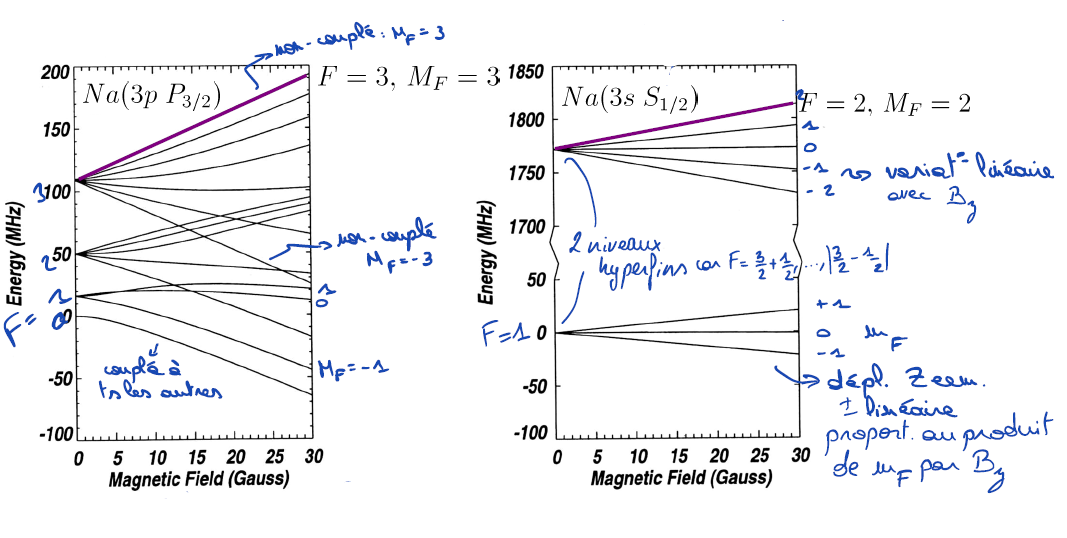
\includegraphics[width=\textwidth]{Images2/ZeemanHyperfin.PNG}
    \caption{Modification des états hyperfins initialement dégénérés en $m_F$ selon le champ magnétique externe $B_z$}
    \label{fig:Zeeman}
\end{figure}
Commençons par le graphe de droite. La subtilité ici est que les deux familles d'états représentés sont très éloignées en énergie et donc n'interagissent quasiment pas (voir théorie des perturbations). On a donc ici le cas simple d'une modification linéaire selon $B_z$ des niveaux d'énergie, ce qui est bien ce qu'on observe. On peut également le comprendre en voyant que la matrice d'interaction ne contient que des termes diagonaux. En effet, les termes non diagonaux sont divisés par le différentiel d'énergie entre les états couplés, il est ici très grand et on néglige donc ces termes.\\

Pour ce qui est du graphe de gauche, il correspond à un autre terme atomique. Ici, à cause de la valeur de spin non nulle, la valeur maximale de $F$ est plus grande et, par conséquent, le nombre d'états de $F$ différents associés à une même valeur de $m_F$ est plus grand. À cause de la proximité en énergie des niveaux, ils vont donc avoir des comportements non linéaires en fonction du champ magnétique $B_z$, car leurs termes non diagonaux ne seront pas négligeables cette fois. On peut le voir aisément pour l'état $(F = 0;m_F = 0)$ qui interagit avec les trois autres états $(F=1,2,3;m_F = 0)$ : son comportement est fortement non-linéaire. On voit également que les états $(F = 3;m_F = \pm3)$ ont bien un comportement linéaire, car ils ne sont couplés avec aucun autre état (ce sont les seuls états ayant $m_F=\pm3$) leurs termes sont donc uniquement diagonaux.\\

Enfin, de manière générale, l'effet de la perturbation entre deux états liés est de créer une répulsion entre eux.




\subsection{Effet Stark}

L'effet Stark est l'équivalent de l'effet Zeeman pour un champ électrique constant dans le temps. Nous allons cependant l'aborder sous un angle légèrement différent grâce à la théorie des perturbations. On définit le moment dipolaire comme suit. On peut se le représenter comme le <<centre de charge>> pris au même sens que le centre de masse de la mécanique classique. $\vec{\epsilon}$ représente le vecteur champ électrique extérieur.

\[
    H \eq H_0 + \lambda H'
\]
\[
    \vec{\mu} \eq \sum_i q_i \vec{r}_i \eq -e\sum_i \vec{r}_i\;\equiv\; \textrm{moment dipolaire}
\]
\[
    H' \eq -\vec{\epsilon}\cdot\vec{\mu}
\]
\[
    \expval{H'} \eq e\bra{\psi}\sum_\imag\vec{r}_i\ket{\psi}\cdot \vec{\epsilon} \eq -\vec{D}\cdot\vec{\epsilon}
\]
En temps normal, un atome isolé n'a pas de moment dipolaire permanent : sa symétrie sphérique l'en empêche. Cependant, sous l'action d'un champ électrique extérieur, ses électrons peuvent se délocaliser : le nuage se déplace dans le sens inverse du champ, entraînant ainsi une polarisation de l'atome. Sous ce champ $E$, notre atome devient donc un dipôle induit.

\[
    \vec{D} \eq \vec{D}_0 + \vec{D}_\text{induit}
\]
\[
    \vec{D}_\text{induit} \eq \alpha \vec{\epsilon} \;\; \text{où}\; \alpha \; \text{est la polarisabilité dipolaire statique de l'atome}
\]
On présente ensuite le développement classique de la théorie des perturbations (cf. Mécanique Quantique 2).

\[
    H\psi_n \eq E_n \psi_n
\]
\[
    E_n \eq \sum_{i=0}^{\infty} \lambda^i E_n^{(i)}\; ; \; \psi_n \eq \sum_{i=0}^{\infty} \lambda^i \psi_n^{(i)}
\]
À l'ordre 0 en $\lambda$, l'Hamiltonien non perturbé correspond aux fonctions de bases à l'ordre 0. L'ensemble des fonctions $\{\psi_k^{(0)}\}$, avec $k$ prenant toutes les valeurs possibles, est donc une base de l'espace des solutions.

\[
    H_0 \psi_n^{(0)} \eq E_n^{(0)} \psi_n^{(0)}
\]
\[
    H_0 \psi_n^{(1)} + H' \psi_n^{(0)} \eq E_n^{(1)} \psi_n^{(0)} + E_n^{(0)} \psi_n^{(1)}
\]
Comme $\{\psi_k^{(0)}\}$ est une base, on peut développer $\psi_n^{(1)}$ sur celle-ci.

\[
    \psi_n^{(1)} \eq \sum_k a_{nk}^{(1)} \psi_k^{(0)}
\]
\[
    \left(H_0 - E^{(0)}_n\right)\sum_k a_{nk}^{(1)} \psi_k^{(0)} + \left(H' - E^{(1)}_n\right)\psi_n^{(0)} \eq 0
\]
On multiplie par le bra $\bra{\psi^{(0)}_l}$, ce qui revient à multiplier par le conjugué de la fonction d'onde associée à $l$ et à intégrer sur $\dif r^3$.

\begin{align*}
    \int \psi^{(0)*}_l\left[ \left(H_0 - E^{(0)}_n\right)\sum_k a_{nk}^{(1)} \psi_k^{(0)} + \left(H' - E^{(1)}_n\right)\psi_n^{(0)}\right] \;\dif r^3 &= a^{(1)}_{nl}(E^{(0)}_l-E^{(0)}_n) \;+\; H'_{ln} - E^{(1)}_n\delta_{ln})\\
    &= 0
\end{align*}
On distingue donc deux cas selon si on se trouve sur la diagonale des éléments de matrice ou non.

\[
    n \eq  l\;:\;\;\; H'_{nn} \eq E^{(1)}_n
\]
\[
    n \neq l\;:\;\;\; a^{(1)}_{nl} \eq \dfrac{H'_{ln}}{E^{(0)}_n-E^{(0)}_l}
\]
On a donc ici une correction diagonale à l'énergie sous la forme de $E^{(1)}_n$ qui ne concerne que l'état lui-même\footnote{A priori, car nous allons voir tout de suite que la symétrie sphérique de l'atome entraîne que cette correction est nulle.} et une correction non diagonale aux vecteurs propres qui fait potentiellement intervenir d'autres états couplés par l'effet Stark avec l'état $n$. On va donc développer à l'ordre deux pour obtenir la correction à l'énergie entraînée par ce couplage.

%il faudrait taper cette partie en LaTeX plutot qu'une image
%À l'ordre 2 en $\lambda$:
%\[
%    H_0 \Psi_n^{(2)} + H'\Psi_n^{(1)} \eq E_n^{(0)}\Psi_n^{(2)} + E_n^{(1)} \Psi_n^{(1)} + E_n^{(2)} \Psi_n^{(0)}
%\]

\begin{figure}[H]
    \centering
    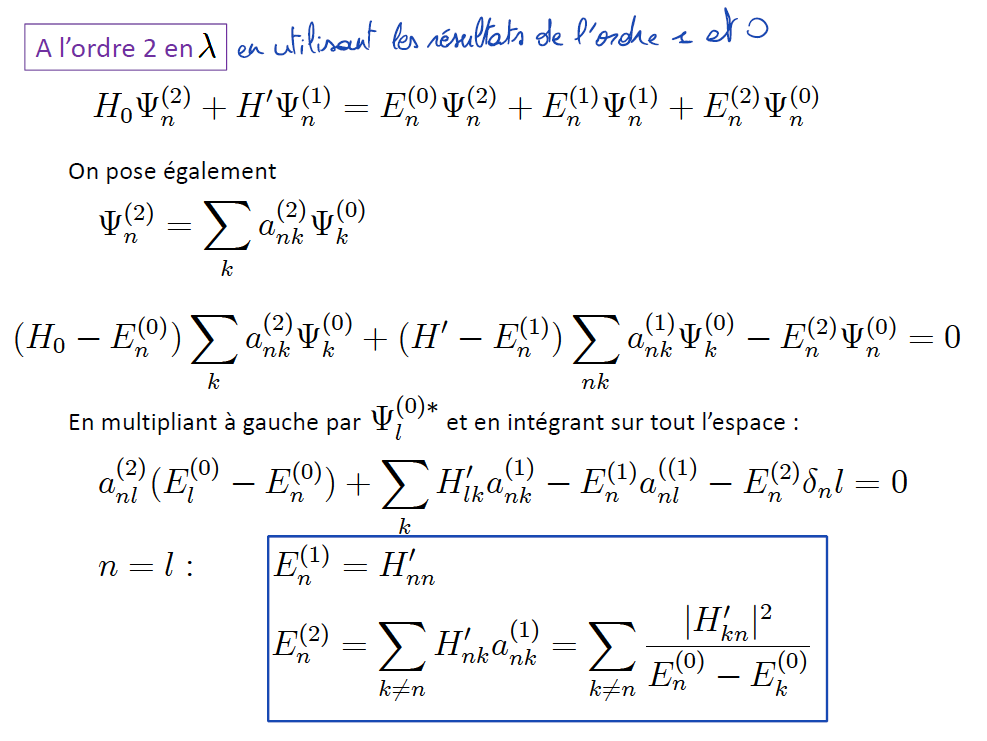
\includegraphics[scale=0.65]{Images2/ordre2.1.PNG}
\end{figure}
On obtient donc $E_n^{(2)}$ qui représente la correction en énergie au second ordre pour le $n^\text{ème}$ état. On voit que, contrairement à la correction au premier ordre qui était diagonale et ne faisait donc intervenir que l'état corrigé, la correction au second ordre n'est pas diagonale et fait donc intervenir d'autres états. On dit que la perturbation couple les états $k$ et $n$ si l'élément de couplage $|H'_{kn}|^2$ n'est pas nul. On regarde ensuite la correction aux vecteurs propres.
\begin{figure}[H]
    \centering
    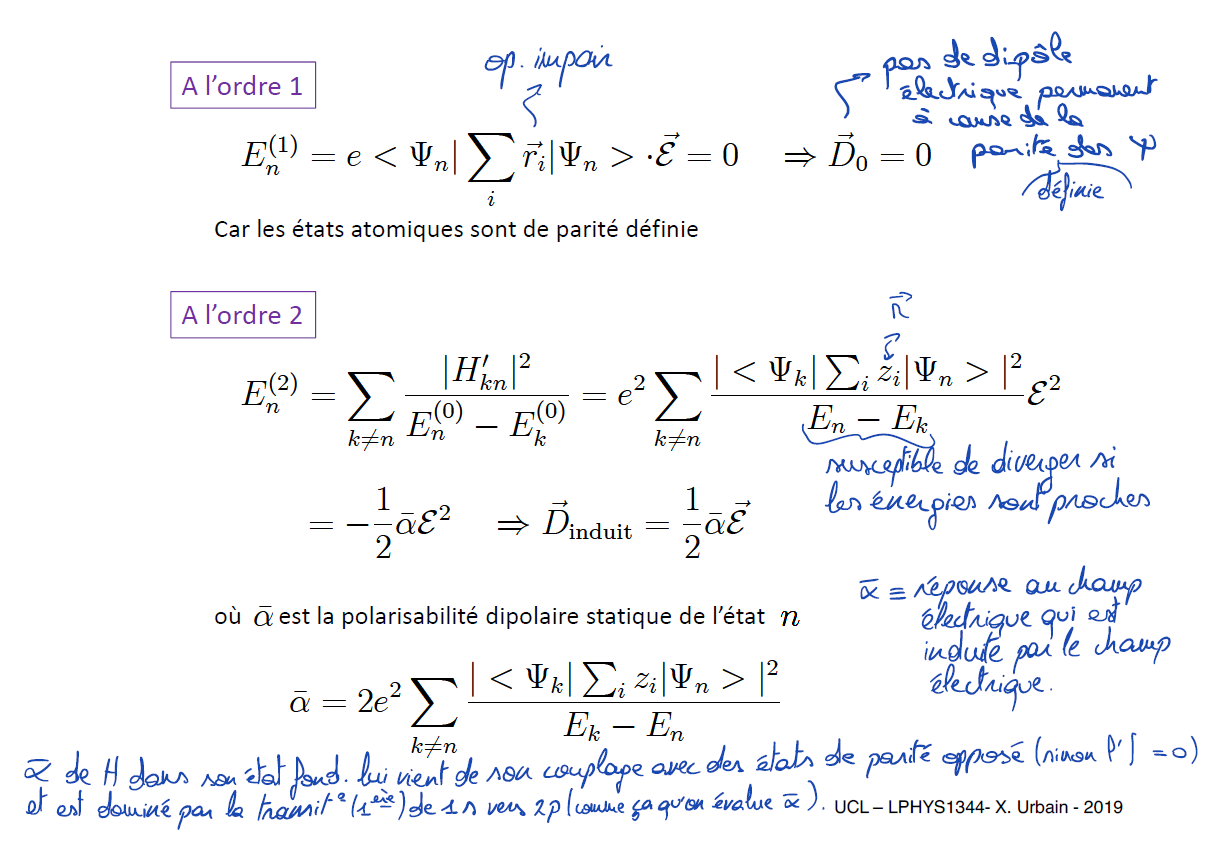
\includegraphics[scale=0.65]{Images2/ordre2.2.PNG}
\end{figure}

En faisant explicitement le calcul de $H'_{nn}$, on fait l'intégrale du produit d'une fonction paire, $|\psi|^2$, et d'une fonction impaire, $\sum_i \vec{r}_i$ : le résultat est donc nul. On retrouve bien le résultat pressenti : un atome ne peut posséder de dipôle permanent, car sa parité est définie, ce qui est une condition analogue ici à présenter une symétrie sphérique.

Par le calcul de la correction à l'énergie au second ordre $E_n^{(2)}$, on a obtenu une expression pour la polarisabilité de l'atome $\bar{\alpha}$.

Pour ce qui est de l'atome d'hydrogène, sa polarisabilité au niveau fondamental vient du couplage de son orbitale s avec des états de parité opposée.



\subsubsection{Cas particulier : états (quasi) dégénérés de parité opposée}

Dans l'atome d'hydrogène, dû à la forte symétrie de sa structure, les états de même $n$ sont tous dégénérés (ce n'est plus le cas dans la structure hyperfine, mais les états demeurent très proches en énergie).

\[
    \ket{nlm}\eq \ket{200},\ket{210},\ket{211},\ket{21\bar{1}}\;\;\text{sont dégénérés}
\]
On représente donc ce mélange d'orbitales de parités différentes par la décomposition sur la base des $\{\psi_{nlm}\}$. Attention on conserve, $m = 0$ car la projection du moment angulaire orbital sur l'axe z doit rester le même. %Honnêtement je suis pas sûr d'avoir compris à 100% pourquoi

\[
    \psi_n^{(0)} \eq \sum_l c_l \psi_{nl0}
\]
On réexprime donc la correction en énergie au premier ordre, le produit scalaire transforme le vecteur de position de l'unique électron $\vec{r}$ en $z$.

\[
    E_n^{(1)} \eq e\bra{\psi_n}z\ket{\psi_n}\epsilon \;\neq \; 0
\]
Grâce à l'hybridation des orbitales, le moment dipolaire permanent de l'hydrogène à l'état fondamental n'est pas nul. En effet, l'opérateur z couple les parties de parité différente de la décomposition de $\psi_n^{(0)}$. Par exemple : $\bra{\psi_{n10}}z\ket{\psi_{n20}}\epsilon \neq 0$.\\

\begin{figure}[H]
    \centering
    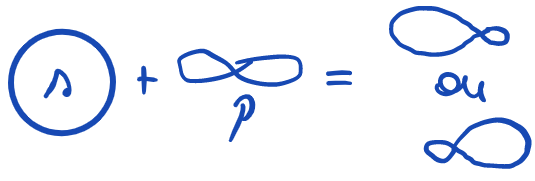
\includegraphics[scale=0.5]{Images2/hybridation.png}
\end{figure}

\textbf{Pour le cas général :}\\

\begin{figure}[H]
    \centering
    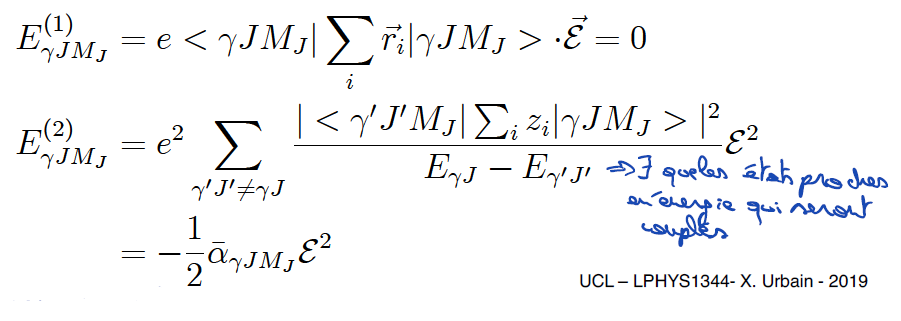
\includegraphics[scale=0.8]{Images2/correcordre.PNG}
\end{figure}

On voit tout de suite que seuls les états proches en énergie seront couplés par la perturbation, ce qui veut explique que l'hybridation d'orbitales dans l'hydrogène fonctionne si bien, car les états hybridés sont (quasi) dégénérés en énergie, on a donc un fort couplage entre eux. En somme, on peut alors parler de polarisabilité de multiplets, car cette notion ne concerne de toute façon que les états d'énergies proches, c'est-à-dire situés dans le même multiplet.\\

On se retrouve donc avec un état fondamental particulier pour l'atome d'hydrogène. Cette particularité sous un champ électrique va nous permettre de réaliser des transitions exotiques. On va par exemple pouvoir réaliser des transitions entre le 2s perturbé (mélange de 2s et 2p) vers l'état 4s (mélange de 4s, 4p, 4d, 4f) ce qui est normalement impossible. On va également pouvoir réaliser des transitions entre ce 2s et le 3s ce qui est normalement impossible à cause de la parité des états.\\

\begin{figure}[H]
    \centering
    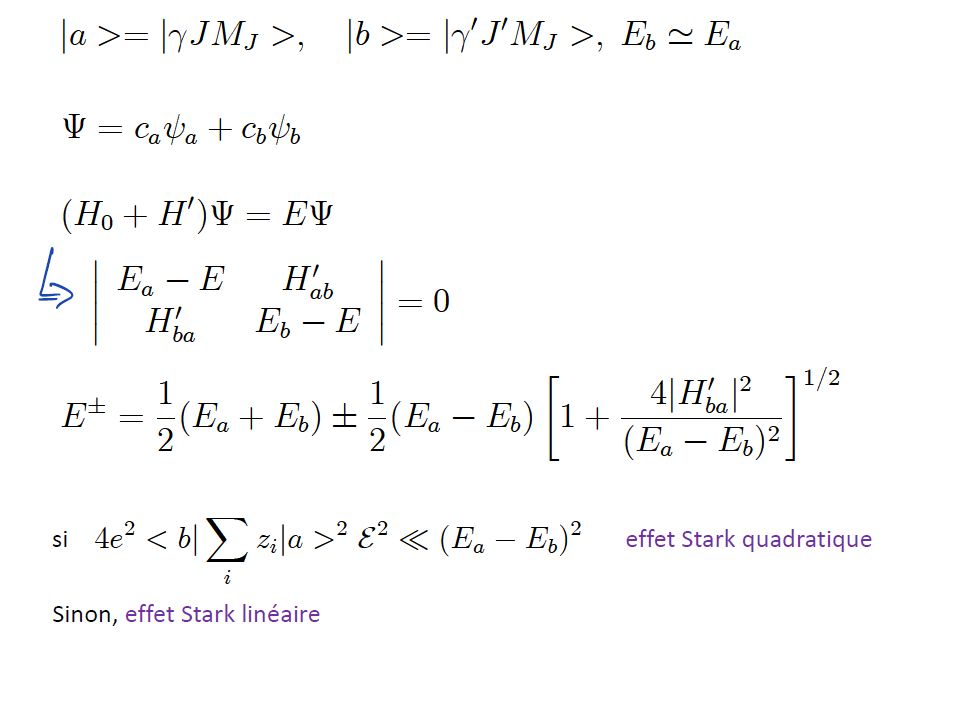
\includegraphics[width=0.65\textwidth]{Images2/EffetStark.PNG}
\end{figure}

On exprime $\psi$ la fonction d'onde sous perturbation comme une combili des $\psi_a$ et $\psi_b$, les fonctions d'onde du système non perturbé. En diagonalisant la matrice de l'Hamiltonien perturbé, on obtient $E^{\pm}$. On distingue deux régimes, soit les énergies sont éloignées $(E_a - E_b)^2 >> 0$ on obtient donc $E^+ = E_a$ et $E^- = E_b$. On a donc pas d'effet pour des énergies très éloignées. Si $4e^2\bra{b}\sum_iz_i\ket{a} = 4|H'_{ba}|^2<<(E_a - E_b)^2 $, par le développement de Taylor de $(1 + x)^2\eq 1 + \dfrac{x}{2} - \dfrac{x^2}{8} + \bigO(x^3)$ ; $x<<1$, on a une modification quadratique en $\epsilon$ des niveaux d'énergie. Si on ne peut pas faire ce raisonnement, on a une évolution linéaire (Fig. \ref{fig:stark_lin}).

\begin{figure}[htp]
    \centering
    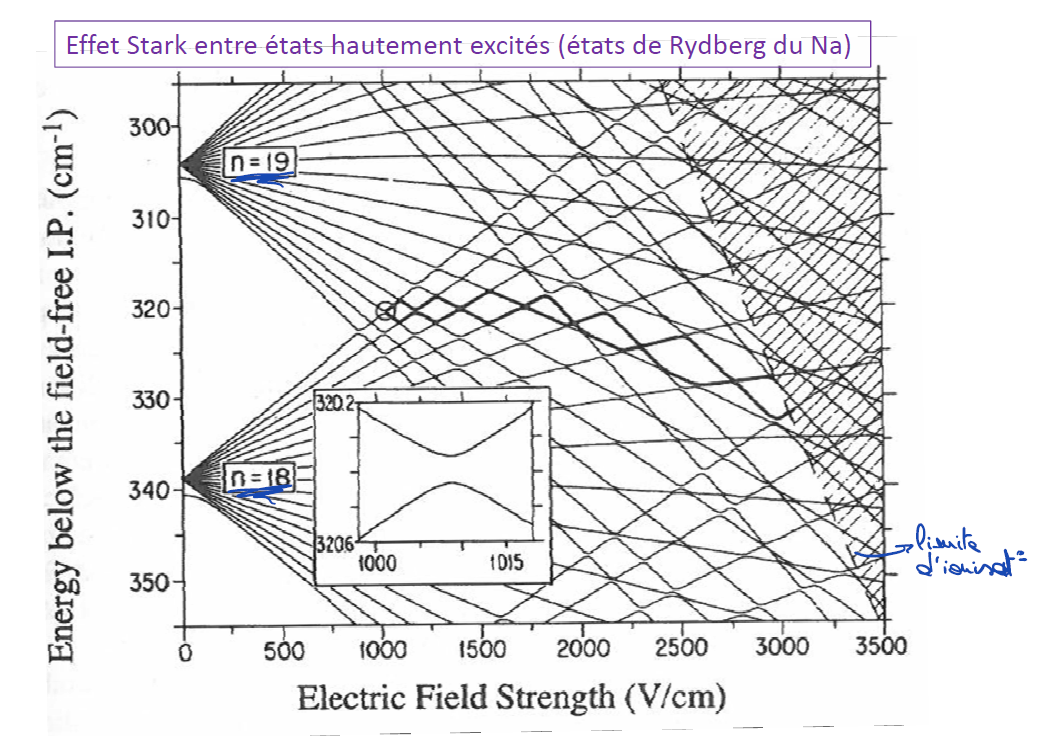
\includegraphics[scale=0.7]{Images2/GrapheStark.PNG}
    \caption{Effet Stark}
    \label{fig:stark_lin}
\end{figure}

On a finalement une évolution en $n^2$ pour l'orbite moyenne (bien qu'il ne s'agisse plus d'orbite de Bohr), la section géométrique ou encore la surface occupée dans l'espace évolue comme le carré du rayon en $n^4$, le moment dipolaire de $L$ à L+1 varie en $n^2$, la polarisabilité en $n^7$, le temps de vie en $n^3$, le moment dipolaire en en $\dfrac{1}{n^4}$ pour le potentiel d'ionisation. Comme la polarisabilité augmente très vite, on peut s'en servir pour guider les atomes via un champ électrique. En condensé :

\[
    a_B \; \propto\; n^2
\]
\[
    S_{at} \; \propto\; n^4
\]
\[
    \mu_\text{dip} \; \propto\; n^2
\]
\[
    \alpha \; \propto\; n^7
\]
\[
    \tau_\text{vie} \; \propto\; n^3
\]
\[
    E_\text{ion} \; \propto\; \dfrac{1}{n^4}
\]

Quand on augmente le nombre quantique principal n, les électrons deviennent moins liés au noyau et donc plus polarisables, l'effet Stark est d'autant plus important. Finalement, pour des $n$ importants, on arrive dans une situation chaotique où les nombres quantiques vont se mélanger et on obtient le genre de graphe présenté au-dessus. À un certain stade, le potentiel coulombien est tellement déformé qu'il laisse s'échapper l'électron comme représenté sur le dessin suivant (Fig. \ref{fig:fig_stark}).\\

\begin{figure}[H]
    \centering
    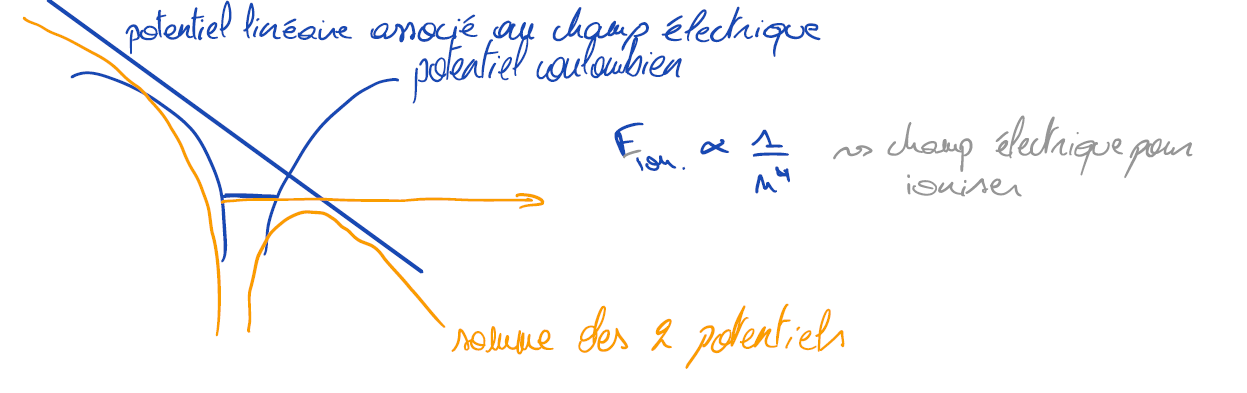
\includegraphics[width=\textwidth]{Images2/DessinStark.PNG}
    \caption{Représentation de l'effet Stark sur le potentiel}
    \label{fig:fig_stark}
\end{figure}
\begin{figure}[H]
    \centering
    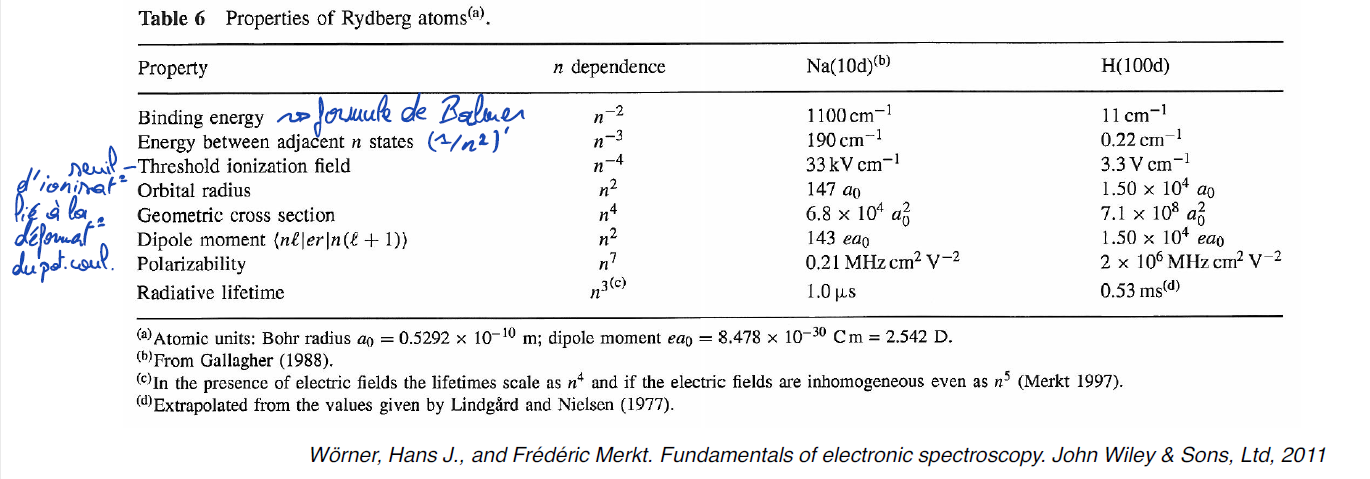
\includegraphics[width=\textwidth]{Images2/TableauStark.PNG}
\end{figure}




\subsubsection{Les aurores boréales}

Dans la haute atmosphère, le $O_2$ entre en collision avec les électrons de haute énergie émis par le soleil. Ces collisions peuvent ioniser $O_2$. La molécule se dissocie ensuite en deux molécules d'oxygène avant de se recombiner

\begin{align*}
    O_2^+ \; + \; e^- \; &\longrightarrow \;O(^3P)\; +\; O(^1S)  \\
    &\longrightarrow\; O(^3P)\; +\; O(^1D)
\end{align*}

Les deux termes excités de même configuration que l'état fondamental sont $^1D$ et $^1S$ (singulet D et singulet S). Chaque processus d'ionisation-recombinaison va produire soit l'un soit l'autre dans certaines proportions mesurables ainsi qu'un $O(^3P)$. On va donc avoir des longueurs d'onde bien précises qui correspondent à deux transitions interdites parce que ces termes sont de même configuration donc forcément de même parité. Dans la cascade de désexcitation de l'oxygène, $^1S$ on va avoir une longueur d'onde de \SI{527}{nm} de couleur verte qui correspond à une transition E2 (quadripolaire électrique, transition interdite) de  $^1S$ vers $^1D$, pas de changement de spin, pas de changement de parité. Un temps de vie de 0.7 seconde est associé à cette transition.\\

Si on regarde la transition du $^1D$ vers le $^3P$, on observe une transition beaucoup plus lente (108 secondes), car on a un changement de spin. Il s'agit donc d'une transition de type M1, dipolaire magnétique avec deux longueurs d'onde possibles, car deux états de J possibles. On a pas accès à, $J=0$ mais $J=1,2$ sont possibles, car on avait $J=2$ dans l'état $^1D$. Dans une phase gazeuse à haute pression donc basse altitude, il est impossible que l'atome passe 108 secondes sans choc avec un autre atome. Par contre à haute altitude, la densité d'atomes est bien inférieure et il devient possible pour un atome de ne rencontrer aucun autre corps sur son temps de désexcitation (108 secondes) et de donc rester exciter jusque émission. Il y a donc une altitude minimale pour une aurore boréale de ce type, sous cette altitude elle change de régime.\\

Résumons : on a une injection de particules chargées le long des pôles (ceinture de Van Allen) par le vent solaire, ce qui va créer un arc le long duquel vont se former les aurores boréales. Les phénomènes d'ionisation-recombinaison émettent des photons à des longueurs bien spécifiques et caractéristiques de transitions interdites dans la molécule d'oxygène. On a deux régimes différents séparés par une limite d'altitude, au-dessus de celle-ci la transition de type M1 (rouge) à long temps de vie a le temps de se faire, car la densité gazeuse est assez faible pour lui permettre de ne heurter aucune autre molécule entre-temps. Sous cette altitude, on observe uniquement la transition E2 de court temps de vie de couleur verte. On a donc dans certains cas, des aurores boréales de couleurs vertes et rouges qui semblent superposées suite à ce phénomène, comme sur la photo.\\

Dans la réalité, il y a bien plus de types d'aurores boréales avec des corps plus lourds comme des molécules ou d'autres atomes.\\

\begin{figure}[htp]
    \centering
    \includegraphics[scale=0.8]{Images2/AuroreBoréale.PNG}
    \caption{Mécanisme des aurores boréales}
    \label{fig:meca_aurores_boreales}
\end{figure}
\begin{figure}[htp]
    \centering
    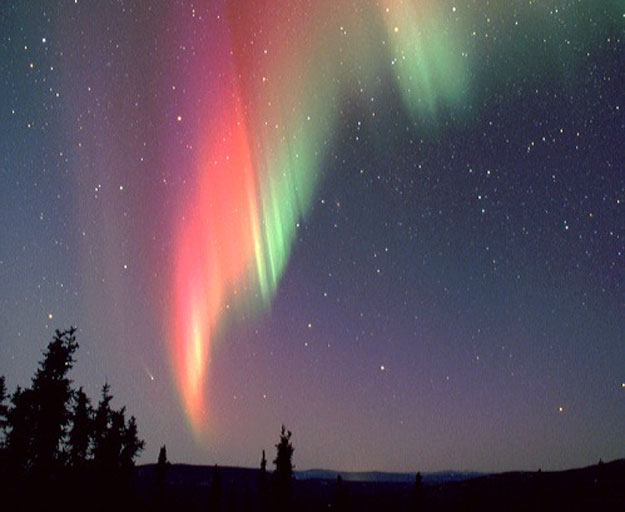
\includegraphics[scale=0.6]{Images2/photoAurore.jpg}
\end{figure}
